\documentclass[12pt,a4paper]{report}

% --- Essential Packages ---
\usepackage[utf8]{inputenc}
\usepackage[T1]{fontenc}
\usepackage[english]{babel}
\usepackage{amsmath, amssymb}
\usepackage{graphicx}
\usepackage{booktabs}
\usepackage{longtable}
\usepackage{pgfplots}
\usetikzlibrary{arrows.meta, positioning, shapes.symbols, fit, calc, backgrounds}
\pgfplotsset{
    compat=1.18,
    % Shared look for the results charts; black/grey styles so they print in greyscale
    resultaxis/.style={
        width=\linewidth, height=7cm,
        grid=major, grid style={gray!30},
        xtick={10,30,50,75},
        tick label style={font=\small}, label style={font=\small}, title style={font=\small},
        legend style={font=\small, at={(0.5,-0.22)}, anchor=north, legend columns=3, draw=none,
            /tikz/every even column/.append style={column sep=0.5cm}},
    },
    algdtac/.style={black, very thick, mark=*},
    algnoscore/.style={black, dashed, mark=o},
    alglru/.style={black, dotted, thick, mark=square*},
    algsieve/.style={gray, thick, mark=triangle*},
    algsfifo/.style={gray, dashdotted, thick, mark=diamond*},
}
\usepackage{setspace}
\usepackage{tocbibind} % Automatically adds lot, lof, bibliography to ToC
\usepackage{hyperref}
\usepackage{parskip}
\usepackage[none]{hyphenat}
\hypersetup{
    colorlinks=true,
    linkcolor=black, % Keeping links black for print quality
    filecolor=black,      
    urlcolor=black,
    citecolor=black,
}
\usepackage{apacite}   % APA style for references
% Italicise "et al." in citations (set at begin-document so apacite's language defaults don't override it)
\AtBeginDocument{%
  \renewcommand{\BOthers}[1]{\textit{et al.}\hbox{}}%
  \renewcommand{\BOthersPeriod}[1]{\textit{et al.}\hbox{}}%
}

% --- Page Layout (Section 1.3) ---
\usepackage{geometry}
\geometry{
    a4paper,
    left=3.7cm,
    right=2.5cm,
    top=2.5cm,
    bottom=2.5cm
}

\usepackage{newtxtext, newtxmath} % Sets global font to Times New Roman

% Note: The requirement "top of the first page of each new chapter, which should be 5.0cm" 
% is usually handled by the default \chapter command in the report class or can be tweaked 
% with the titlesec package if exact 5.0cm from the absolute top edge is strictly enforced.
\usepackage{titlesec}

% --- Chapter Heading ---
% Centered, 14pt, Bold, format: "CHAPTER ONE" with the title on the next line
\usepackage{fmtcount}
\newcommand{\chapnum}{\NUMBERstring{chapter}} % chapter number in words; appendices switch back to letters
\titleformat{\chapter}[display]
  {\normalfont\fontsize{14}{17}\bfseries\centering}
  {\MakeUppercase{\chaptertitlename}\ \chapnum}
  {0pt}
  {\MakeUppercase}
% Remove extra top and bottom spacing around chapter titles
\titlespacing*{\chapter}{0pt}{0pt}{1\baselineskip} 

% --- Level One Heading (Section) ---
% Left aligned, 14pt, Bold
\titleformat{\section}
  {\normalfont\fontsize{14}{17}\bfseries}
  {\thesection}
  {1em}
  {}

% --- Level Two Heading (Subsection) ---
% Left aligned, 12pt (normalsize since doc is 12pt), Bold
\titleformat{\subsection}
  {\normalfont\normalsize\bfseries}
  {\thesubsection}
  {1em}
  {}

% --- Level Three Heading (Subsubsection) ---
% Left aligned, 12pt, Bold, Italicised
\titleformat{\subsubsection}
  {\normalfont\normalsize\bfseries\itshape}
  {\thesubsubsection}
  {1em}
  {}

% --- Title Page Variables ---
\title{\MakeUppercase{Dynamic Traffic-Aware Web Caching: Implementing Heuristic Routing to Mitigate AI Scraper Interference}}
\author{\MakeUppercase{Joseph Alikah}}
% Add custom commands for specific title page requirements
\newcommand{\matriculation}{231414}
\newcommand{\degree}{Bachelor of Science}
\newcommand{\submissionmonth}{September 2026}

\begin{document}

% --- 1.2 Title Page ---
\begin{titlepage}
    \begin{center}
        \vspace*{1.5cm}

        
\includegraphics[width=2cm]{figures/UI_logo.png}
        
        \vspace{1.5cm} % Space between logo and title
        
        \textbf{\Large \MakeUppercase{Dynamic Traffic-Aware Web Caching: Implementing Heuristic Routing to Mitigate AI Scraper Interference}}\\
        \vspace{1.5cm}
        
        \textbf{\MakeUppercase{Joseph Alikah}}
        
        \vspace{0.5cm}
        Matriculation Number: 231414
        
        \vspace{1.5cm}
        
        Supervised by\\
        \vspace{0.5cm}
        \textbf{Dr. Nancy Woods}
        
        \vspace{1.5cm}
        
        In Partial Fulfilment to Requirements for the Award of the Degree of\\
        \vspace{0.5cm}
        \textbf{Bachelor of Science (B.Sc.) in Computer Science}
        
        \vspace{1.5cm}
        
        Department of Computer Science\\
        Faculty of Science\\
        University of Ibadan, Ibadan, Nigeria
        
        \vfill
        
        \textbf{November 2026}
    \end{center}
\end{titlepage}

% --- Front Matter ---
\pagenumbering{roman}
\setcounter{page}{1} % Often starts at ii after title page
\doublespacing
\noindent

% --- 1.6 Certification ---
\chapter*{Certification}
\addcontentsline{toc}{chapter}{Certification}
This is to certify that this research work was carried out by \textbf{ALIKAH, Joseph Ehiagwina}
with matriculation number \textbf{231414} in the Department of Computer Science, University of Ibadan.
This research work is considered adequate in partial fulfilment of the requirements for the award
of a Bachelor of Science in Computer Science.

\vspace{3cm}
\noindent
\begin{tabular*}{\textwidth}{@{} l @{\extracolsep{\fill}} c @{}}
\rule{6cm}{1pt} & \rule{4cm}{1pt} \\
\textbf{Dr. Nancy Woods} & \textbf{Date} \\
Project Supervisor & \\
Department of Computer Science & \\
\end{tabular*}

\vspace{3cm}
\noindent
\begin{tabular*}{\textwidth}{@{} l @{\extracolsep{\fill}} c @{}}
\rule{6cm}{1pt} & \rule{4cm}{1pt} \\
\textbf{Prof. Bolanle Oladejo} & \textbf{Date} \\
Head of Department (HOD) & \\
Department of Computer Science & \\
\end{tabular*}

\newpage

% --- 1.7 Dedication ---
\chapter*{Dedication}
\addcontentsline{toc}{chapter}{Dedication}
\noindent

This report is dedicated to God, whose guidance and blessings have enabled me to navigate
through the challenges and achieve my goals.

I also dedicate this work to my parents, Dr. Sylvester Alikah and Dr. Anita Alikah, whose
unwavering support, encouragement, and sacrifices have been the bedrock of my academic and
personal growth. Their belief in my potential has been a constant source of motivation.

\newpage

% --- 1.8 Acknowledgements ---
\chapter*{Acknowledgements}
\addcontentsline{toc}{chapter}{Acknowledgements}
\noindent

First and foremost, I would like to express my deepest gratitude to my project supervisor,
Dr. Nancy Woods, for her invaluable guidance, patience, and continuous support throughout
this research. Her expertise and constructive feedback were instrumental in shaping this
thesis and ensuring its successful completion.

I also extend my sincere appreciation to all my lecturers in the Computer Science Department.
Your dedication to teaching, insightful mentorship, and commitment to academic excellence
have profoundly shaped my educational journey and prepared me for the future.

To my friends and classmates, thank you for the late-night study sessions, the shared laughter,
and the mutual encouragement. Navigating the rigors of this degree would not have been the
same without your camaraderie.

Furthermore, I am endlessly grateful to my parents, Dr. Sylvester Alikah and Dr. Anita Alikah,
and my extended family. While this work is dedicated to you, I want to acknowledge once again
the emotional and financial support you have provided. Thank you for always believing in my
vision and for giving me the foundation I needed to succeed.

Finally, I give thanks to God for the grace, wisdom, and strength granted to me throughout
my entire academic endeavour.

\newpage

% --- 1.12 Abbreviations (Moved before ToC as per spec) ---
\chapter*{List of Abbreviations}
\addcontentsline{toc}{chapter}{List of Abbreviations}
\begin{longtable}{@{}ll}
\textbf{Abbreviation} & \textbf{Full Meaning} \\
\endhead
AI & Artificial Intelligence \\
API & Application Programming Interface \\
ARC & Adaptive Replacement Cache \\
ASN & Autonomous System Number \\
AUC & Area Under the Curve \\
BHR & Byte Hit Rate \\
CDF & Cumulative Distribution Function \\
CDN & Content Delivery Network \\
CHR & Cache Hit Ratio \\
CI & Confidence Interval \\
CPI & Cache Pollution Index \\
CPU & Central Processing Unit \\
DDoS & Distributed Denial of Service \\
DNN & Deep Neural Network \\
DTAC & Dynamic Traffic-Aware Cache \\
EWMA & Exponentially Weighted Moving Average \\
FIFO & First-In, First-Out \\
FPR & False-Positive Rate \\
GMM & Gaussian Mixture Model \\
HTTP & Hypertext Transfer Protocol \\
IP & Internet Protocol \\
JSON & JavaScript Object Notation \\
LFU & Least Frequently Used \\
LLM & Large Language Model \\
LLR & Log-Likelihood Ratio \\
LRU & Least Recently Used \\
NAT & Network Address Translation \\
OSI & Open Systems Interconnection \\
RAG & Retrieval-Augmented Generation \\
ROC & Receiver Operating Characteristic \\
RSS & Resident Set Size \\
S3-FIFO & Simple, Scalable, Scan-resistant FIFO \\
SEO & Search Engine Optimization \\
SSD & Solid State Drive \\
TLS & Transport Layer Security \\
VPN & Virtual Private Network \\
\end{longtable}
\newpage

% --- 1.10 Table of Contents ---
\tableofcontents
\newpage

% --- 1.11 List of Tables, Figures, Plates ---
\listoftables
\newpage
\listoffigures
\newpage
% Custom list of plates if necessary, often combined with figures or created using float package.

% --- 1.9 Abstract ---
\chapter*{Abstract}
\addcontentsline{toc}{chapter}{Abstract}

Traditional web caching relies on the natural Zipfian distribution and temporal locality of human browsing to efficiently store popular content at the network edge. However, the explosive growth of Artificial Intelligence (AI) scrapers harvesting training data has fundamentally disrupted this ecosystem. These automated bots generate high-volume, non-recurring scan patterns that break traditional eviction policies like Least Recently Used (LRU). Consequently, scraper traffic induces severe cache pollution, prematurely flushing legitimate content and drastically degrading overall infrastructure performance.

To address this vulnerability, this study designs and implements a Dynamic Traffic-Aware Cache (DTAC) in Rust. A lightweight Heuristic Proxy evaluates passive signals (per-IP request velocity, missing browser headers, the absence of auxiliary asset fetches, and datacenter network origin) and combines them in a log-odds model into a continuous bot-probability score for every request, at a bounded per-request cost. The cache engine weights each request's contribution to a resource's decaying popularity score by how human the request appears, and uses that score both to admit resources from a metadata-only ghost cache and to choose eviction victims through a randomized sampling tournament.

DTAC was benchmarked against LRU, the scan-resistant SIEVE and S3-FIFO algorithms, and an ablation of itself that ignores the score, in 350 replays of synthetic traffic that mixed Zipf-distributed human browsing sessions with 10--75\% scraper traffic over five random seeds. Against scrapers with detectable signatures, the router separated bots from humans perfectly, and at a cache size of 10\% of the catalog DTAC's human hit rate stayed at 58.2--58.3\% regardless of the bot share. At 75\% bot traffic it exceeded LRU by 17.1 percentage points, SIEVE by 3.9, S3-FIFO by 5.1 and its own ablation by 4.3, admitted no bot-only content, and added about 23--39 microseconds of scoring time at the 99th percentile. Against stealthy scrapers that imitate browsers, the heuristics performed no better than chance and DTAC matched its ablation, still outperforming LRU and S3-FIFO. At a cache size of 20\% of the catalog DTAC fell behind SIEVE. The results show that a bot-probability score can substantially protect human cache performance in a single shared cache, and that its value depends on how well the score identifies the bots.

% UI does not need keywords
% \vspace{1cm}
% \noindent\textbf{Keywords:} Keyword 1, Keyword 2, Keyword 3, Keyword 4, Keyword 5. % 3 to 5 keywords
\newpage

% --- Main Body ---
\pagenumbering{arabic}
\doublespacing % Often required for thesis, adjust if 1.5 spacing is preferred.

% Include Chapters (1.13 General Structure)
\chapter{Introduction}
\label{chap:introduction}

\section{Background to the Study}

\subsection{Historical Web Caching and Human Traffic Distributions}
Web caches are fundamental infrastructure systems designed to reduce web server load and latency by storing resources geographically and network-wise closer to the user \cite{breslau_web_1999}. By serving repeated requests from intermediate storage, caching prevents the need to fetch content directly from the origin web server on every individual request \cite{breslau_web_1999, umar_experimental_2026}. Historically, web caching algorithms have been highly effective because human browsing patterns naturally follow the Zipfian law, where a small set of popular web pages are requested frequently while the vast majority are accessed rarely \cite{breslau_web_1999}. Because human traffic exhibits high temporal locality, where recently accessed data is highly likely to be requested again in the near future, caching systems can easily store popular content at the network edge. This strong human locality of reference established the theoretical and practical foundation for traditional caching eviction policies, such as the Least Recently Used (LRU) algorithm \cite{breslau_web_1999}.

\subsection{The Proliferation of AI Scrapers and Crawlers}
However, the modern web ecosystem has experienced a massive influx of Artificial Intelligence (AI) scrapers and automated crawlers designed to harvest vast quantities of web data for training machine learning models and large language models (LLMs) \cite{kim_scrapers_2025, zhang_rethinking_2026}. While automated web crawlers have existed for decades, historically utilized for search engine indexing and search engine optimization (SEO), the explosive growth of AI has fundamentally altered the threat landscape and the sheer scale of network traffic \cite{kim_scrapers_2025}. Today, aggressive AI data scrapers and live-retrieval crawlers overwhelm network edges to build massive training corpora or power retrieval-augmented generation (RAG) tasks \cite{zhang_rethinking_2026}.

\subsection{The Disruption of the Caching Ecosystem}
Unlike human users, these AI scrapers typically make high-volume, singular, and non-recurring requests across wide swaths of web pages that will never be requested again \cite{zhang_rethinking_2026}. This behavior fundamentally breaks the Zipfian distribution pattern that traditional caching algorithms rely upon. Automated bots generate what is known as a "scan" pattern: a request stream that touches a large number of distinct objects with little-to-no reuse in a short period, replacing the varied and deep browsing habits of humans with superficial single accesses \cite{zhang_rethinking_2026}. Consequently, current caching algorithms fail to handle this uniform, non-recurring traffic effectively. When traditional caches are subjected to these scan patterns, the algorithms are effectively flushed, causing cache hit ratios to decline steeply and leading to severe operational inefficiencies \cite{zhang_rethinking_2026}.

\subsection{The Evasion of Passive Defenses}
Furthermore, mitigating this aggressive automated traffic is severely complicated by the evasion tactics of modern bots. Recent empirical studies demonstrate that modern AI scrapers selectively ignore standard voluntary domain directives such as robots.txt, rendering passive exclusion policies highly unreliable \cite{kim_scrapers_2025}. When web administrators attempt to enforce active, friction-based defenses like CAPTCHAs or behavioral biometrics, modern AI systems quickly bypass them using sophisticated deep learning solvers and reinforcement learning agents designed to mimic human environmental characteristics \cite{ousat_broken_2026}. Because automated systems actively evade traditional security measures while simultaneously breaking the foundational assumptions of temporal locality, web caches remain critically vulnerable to AI-induced infrastructure degradation.

\section{Statement of the Problem}
The fundamental problem addressed by this study is that high-volume, non-recurring scan patterns generated by modern Artificial Intelligence (AI) scrapers induce severe cache pollution, forcing traditional eviction algorithms to prematurely discard frequently accessed human content which ultimately degrades system performance, inflates origin server loads, and increases latency for legitimate users \cite{zhang_rethinking_2026}.

\section{Aims and Objectives}

\subsection{Primary Aim}
The primary aim of this research is to design and implement a dynamic, heuristic caching architecture that mitigates Artificial Intelligence (AI) scraper interference and preserves web cache efficiency \cite{zhang_rethinking_2026}.

\subsection{Specific Objectives}
To achieve this aim, the specific objectives of the study are to:
\begin{itemize}
    \item Build a lightweight heuristic detector utilizing passive network analysis, specifically evaluating HTTP header anomalies and structural requests \cite{van_boxem_shy_2026}.
    \item Assign a real-time, continuous "AI-score" ranging from 0.0 to 1.0 to incoming HTTP requests, at a bounded per-request cost that does not grow with traffic volume, to probabilistically quantify automated bot origins \cite{chandra_composite_2026, van_boxem_shy_2026}.
    \item Develop a Dynamic Traffic-Aware Cache (DTAC) architecture whose admission and eviction decisions are weighted by the assigned real-time AI-scores, in place of the score-blind recency ordering of the standard Least Recently Used (LRU) algorithm \cite{zhang_rethinking_2026}.
    \item Evaluate the DTAC prototype by benchmarking its cache hit rates against standard LRU and the scan-resistant SIEVE and S3-FIFO algorithms under controlled, simulated workloads of mixed human and AI traffic \cite{breslau_web_1999, zhang_rethinking_2026}.
\end{itemize}

\section{Scope of the Research}

\subsection{Architectural Boundaries}
This study is strictly focused on server-side web caching infrastructure and routing optimization in the presence of automated scraping workloads \cite{umar_experimental_2026, zhang_rethinking_2026}. Architecturally, the research is bounded by the design and implementation of a two-stage system. This system comprises a Heuristic Proxy (featuring a State Manager and an AI-Score Generator) and a Dynamic Traffic-Aware Cache (DTAC) positioned upstream of an origin web server \cite{van_boxem_shy_2026, zhang_rethinking_2026}. The scope excludes the development or integration of client-side bot detection mechanisms, such as CAPTCHAs or behavioral biometrics, focusing entirely on passive, network-layer routing.

\subsection{Methodological Scope}
The methodological scope of this research is strictly constrained by the latency and concurrency requirements of edge-proxy environments, necessitating algorithms whose per-request cost is small and bounded, independent of the volume of traffic observed. Consequently, the proxy's threat evaluation is bounded to passive, Application Layer (OSI Layer 7) HTTP/HTTPS traffic analysis, utilizing Bayesian-style probability (Log-Odds classification) and bitwise Exponentially Weighted Moving Averages (EWMA) to assess behavioral metadata such as request velocity and structural anomalies. The integration of computationally heavy machine learning models, such as Deep Neural Networks (DNNs), directly on the critical path is explicitly excluded to avoid unacceptable latency spikes. Furthermore, the methodology is designed specifically to mitigate application-layer AI scrapers and cache-polluting botnets; thus, the mitigation of lower-level volumetric DDoS attacks (OSI Layers 3 and 4) falls outside the purview of this study, operating under the assumption that standard upstream infrastructure handles such threats.

To ensure system stability under internet-scale traffic, the methodology enforces strict bounded-memory constraints, intentionally abandoning unbounded state tracking and globally sorted cache queues. Client state tracking is limited to the probabilistic Space-Saving algorithm, while cache eviction relies entirely on lazy evaluation via randomized sampling (the ``Power of N Choices'') and lock-sharded metadata tracking utilizing a dual-stage Ghost Cache. The evaluative scope of this architecture is bounded to measuring cache hit rate, byte hit rate, cache pollution, memory consumption, and per-request latency. Validation is conducted entirely through synthetic traffic models that combine Zipfian (heavy-tailed) human browsing sessions with two classes of scraper traffic: ``naive'' scrapers that exhibit the mechanical signatures the heuristics target, and ``stealthy'' scrapers that imitate browsers in order to probe where those heuristics stop working. The study assesses the system's ability to reduce the cache admission of automated traffic while preserving cache capacity for legitimate users; evaluation on real production traffic is outside its scope.

\section{Justification for the Research}

\subsection{The Failure of Current Mitigations}
The exponential growth of large language models and AI tools has driven a corresponding surge in web scraping activity \cite{zhang_rethinking_2026}. Because empirical evidence confirms that AI scrapers routinely ignore voluntary compliance mechanisms like robots.txt, web administrators can no longer rely on protocol-based exclusion to protect their infrastructure \cite{kim_scrapers_2025}. Furthermore, current active mitigation strategies, such as CAPTCHAs and behavioral biometrics, degrade user experience and are increasingly bypassed by modern automated solvers \cite{ousat_broken_2026}. While architectural solutions like physically partitioning hardware for different traffic types (split caches) offer isolation, they introduce severe resource fragmentation and economic inefficiencies that are impractical for most small-to-medium platforms \cite{zhang_rethinking_2026}.

\subsection{Protection of Infrastructure and Cost Efficiency}
This research is justified by its direct utility in safeguarding web performance \cite{umar_experimental_2026}. While network-level defenses such as hierarchical IP hashing exist to mitigate high-volume scraper strain \cite{hoetzlein_protecting_2025}, server-side caching systems themselves must be architecturally modernized to survive modern traffic anomalies. By introducing an AI-aware heuristic eviction mechanism, the proposed DTAC system proactively protects human traffic by preserving the temporal locality benefits of caching for actual end users \cite{breslau_web_1999, zhang_rethinking_2026}. Where scraper traffic can be distinguished from human traffic, such a system can sustain higher cache hit rates for human users during periods of heavy scraper congestion, thereby saving server compute, bandwidth, and operational costs.
\chapter{Literature Review}

\label{chap:literature_review}

\section{Introduction}
The rapid proliferation of large language models (LLMs) and artificial intelligence agents has fundamentally altered the landscape of web traffic. Historically, web infrastructure and caching architectures were optimized for human browsing behavior, which relies heavily on predictable temporal locality and repetitive access to popular content. Today, aggressive AI data scrapers and live-retrieval crawlers overwhelm network edges with sequential, non-repeating ``scan'' patterns that actively degrade traditional cache performance, evicting high-value human data and driving up backend server costs.

While solutions exist in isolation (such as physically partitioning cache hardware for different traffic types, or employing active bot challenges like CAPTCHAs), they introduce severe trade-offs. Active challenges impose unacceptable latency and privacy concerns, while hardware partitioning causes resource fragmentation that is economically unfeasible for small-to-medium web platforms. Consequently, there is a critical need for a unified caching architecture that dynamically incorporates real-time, lightweight bot-probability scores into its eviction logic, safely penalizing scraper traffic without sacrificing the shared resource pool.

To establish the theoretical and technical foundation for this proposed architecture, this literature review examines three core areas at the intersection of network security and systems memory management. The scope of this chapter is structured as follows:

\begin{itemize}
    \item \textbf{Section 2.2 (The Impact of AI Scrapers on Web Infrastructure)} defines the modern threat landscape, detailing how automated LLM data collection breaks the foundational assumptions of human web traffic distributions.
    \item \textbf{Section 2.3 (Existing Mitigation Strategies and Resource Partitioning)} evaluates current architectural solutions, specifically highlighting the operational flaws and hardware inefficiencies of physically split caches.
    \item \textbf{Section 2.4 (Traffic Classification and Bot Heuristics)} reviews the evolution of bot detection, showing that it is feasible to assign an aggregate ``AI-score'' at a small, bounded per-request cost using passive, lightweight network heuristics.
    \item \textbf{Section 2.5 and beyond (Cache Eviction Algorithms)} explores the progression from traditional eviction policies (such as LRU and LFU) to modern, scan-resistant algorithms (such as ARC, S3FIFO, and SIEVE), ultimately identifying the research gap for integrating probabilistic trust scores directly into state-of-the-art eviction engines.
\end{itemize}

By synthesizing these domains, this review demonstrates that while the tools for low-latency bot detection and scan-resistant caching exist independently, they have not yet been bridged to form a dynamic, AI-aware cache eviction policy.

\section{The Impact of AI Scrapers on Web Infrastructure}
To understand why modern web caching systems are failing under the weight of automated traffic, it is necessary to examine how the fundamental assumptions of web request distributions have been disrupted. This section outlines the historical baseline of human web traffic, the evolution of automated agents, and how the specific access patterns of large language model (LLM) scrapers actively degrade caching infrastructure.

\subsection{Historical Context: Human Traffic and Temporal Locality}
Traditional web cache architectures were designed around the predictable nature of human browsing. Foundational research demonstrated that human web requests follow a Zipf-like distribution, meaning a small number of popular web objects receive the vast majority of requests, while a ``long tail'' of objects are accessed infrequently \cite{breslau_web_1999}. 

Because human traffic exhibits high temporal locality, where recently accessed data is highly likely to be requested again in the near future, caching systems could easily store popular content at the network edge to reduce server load and latency. As long as traffic predominantly adhered to this Zipfian model, traditional eviction algorithms performed exceptionally well.

\subsection{The Modern Web Landscape: The Rise of AI Bots}
In the modern era, the web is no longer exclusively navigated by humans. While web scrapers and crawlers are ``nearly as old as the internet'' \cite{kim_scrapers_2025}, their purpose and scale have evolved. Early automated traffic was largely driven by search engine indexers and marketing bots analyzing Search Engine Optimization (SEO), which became a crucial mechanism for digital marketing \cite{berman_role_2012}.

However, the explosive growth of artificial intelligence has fundamentally altered the threat landscape. \citeA{kim_scrapers_2025} define crawling as ``the process of systematically accessing links on the web,'' and scraping as ``the act of downloading information from each link.'' They note that ``interest in data scraping has only increased as AI models have grown in size and scope.'' Today, automated web traffic includes highly aggressive LLM training bots and live-retrieval AI agents that place unprecedented strain on web infrastructure.

\subsection{AI Bot Access Patterns: The ``Scan'' Problem}
The core issue with modern AI bots is that their access patterns are entirely antithetical to the Zipf-like distributions that caches rely on. \citeA{zhang_rethinking_2026} categorize modern AI bots into two distinct groups, both of which severely disrupt caching:

\begin{itemize}
    \item \textbf{AI Data Scrapers:} These bots focus on ``harvesting data to build large training corpora for models like LLMs.'' They exhibit exceptionally high unique access ratios. Data from large-scale legitimate web crawls confirms that the vast majority of fetched pages are entirely unique, prioritizing breadth over repetition.
    \item \textbf{AI Search Crawlers:} These bots fetch content to support live AI services, such as retrieval-augmented generation (RAG) for answering questions. They ``rely on accessing a broad set of unique pages to achieve better task performance,'' generating high-volume traffic with low reuse.
\end{itemize}

Both categories generate what \citeA{zhang_rethinking_2026} define as a scan pattern: ``a request stream that touches a large number of distinct objects with little-to-no reuse in a short period.'' This observation aligns with earlier behavioral analyses by \citeA{alnoamany_access_2013}, who found that while human browsing is varied and deep, automated robots are limited almost exclusively to superficial ``Dips'' (single accesses) and ``Skims'' (fetching lists of available pages).

When caching algorithms process these scan patterns, the results are catastrophic for performance. \citeA{zhang_rethinking_2026} found that under pure Zipfian (human) traffic, standard algorithms achieve 70--80\% hit rates. However, ``as the fraction of AI traffic increases, hit rates decline steeply, falling below 30\% for all policies at a 75\% scan ratio.'' Scrapers effectively flush the cache, evicting high-value, frequently requested human content in favor of single-use data that will not be requested again.

\subsection{The Failure of Voluntary Compliance and Traditional Defenses}
Mitigating these aggressive scan patterns is complicated by the fact that modern bots frequently evade both voluntary guidelines and traditional security measures.

Historically, web administrators relied on the \texttt{robots.txt} protocol to dictate which parts of a site could be crawled. However, \citeA{kim_scrapers_2025} found that modern bots selectively ignore these directives. Stricter directives correlate with lower compliance, and ``certain categories of bots, including AI search crawlers, rarely check \texttt{robots.txt} at all,'' rendering voluntary compliance mechanisms highly risky and unreliable.

When administrators implement active defenses, modern AI systems quickly adapt. \citeA{ousat_broken_2026} stress that ``many deployed defenses are fragile under composition attacks.'' Their research highlights that traditional web bot management systems are highly vulnerable to automated solvers:
\begin{itemize}
    \item Text-based challenges have been defeated by Generative Adversarial Networks (GANs) and Convolutional Neural Networks (CNNs) with success rates exceeding 94\%.
    \item Image-based challenges (like reCaptcha) have been bypassed by deep learning solvers exploiting image repetition with 70\% accuracy.
    \item Behavioral scoring systems (like reCaptcha v3) have been compromised using reinforcement learning agents trained to simulate human-like browsing, achieving evasion rates up to 99.6\%.
\end{itemize}

Because AI scrapers ignore voluntary protocols, easily bypass traditional friction-based security, and fundamentally break standard caching algorithms, there is a critical need for alternative infrastructure defenses that operate passively at the caching layer.

\section{Existing Mitigation Strategies and Resource Partitioning}
As the strain of automated AI traffic on web infrastructure grows, several mitigation strategies have been proposed. These range from network-layer blocking to architectural redesigns of caching tiers. However, existing solutions often introduce unacceptable trade-offs in accuracy, cost, or hardware efficiency, highlighting the need for a more dynamic approach.

\subsection{Strict Bot Blocking and Rate Limiting}
The most direct response to aggressive automated traffic is strict blocklisting or aggressive rate limiting at the network edge. However, in the modern web ecosystem, blocking all bots is largely infeasible. Overly aggressive blocking mechanisms inevitably produce false positives, incorrectly blocking legitimate human users and degrading the user experience. Furthermore, not all automated traffic is malicious or unwanted; benign bots, such as search engine indexers and SEO crawlers, are critical for a domain's visibility and discoverability. Consequently, mitigation strategies cannot rely purely on binary blocking; they must allow some automated traffic while mitigating its impact on infrastructure.

\subsection{Scan-Resistant Eviction Algorithms}
Recognizing that strict blocking is imperfect, recent research has explored how cache eviction policies themselves can absorb the impact of AI scrapers. Traditional policies like Least Recently Used (LRU) and Least Frequently Used (LFU) degrade rapidly under scan-heavy traffic. However, algorithms designed to penalize ``one-hit wonders'' offer better resilience.

\citeA{zhang_rethinking_2026} evaluated state-of-the-art eviction algorithms and found that policies like SIEVE, S3FIFO, and ARC perform significantly better under scraper loads. They note that these policies ``maintain over 75\% hit rate for human requests even when scan ratio reaches 50\%, whereas simpler strategies like LRU, LFU, and FIFO degrade more quickly.'' Ultimately, Zhang \textit{et al.}\ conclude that ``smarter eviction algorithms can serve as lightweight traffic filters'' offering an additional layer of protection against AI interference.

While these advanced algorithms are an improvement, they are fundamentally naive to the origin of the request. They infer bot-like behavior purely from access patterns (recency and frequency) after the cache is already under pressure. Integrating explicit AI detection scores into the eviction logic presents a clear avenue to improve upon the state-of-the-art, proactively preserving hit rates before human data is evicted.

\subsection{Hardware Partitioning and Split Caches}
To prevent AI traffic from overwhelming main servers and edge caches, \citeA{zhang_rethinking_2026} propose a ``composable caching hierarchy that coordinates differentiated tiers for human and AI workloads.'' Instead of a single shared cache, this architecture uses overlapping cache tiers with distinct roles. To balance performance and cost, they recommend that ``human traffic should continue to be served primarily from edge caches optimized for low latency and high hit rates,'' while AI requests are routed to separate, deeper storage tiers.

This split-cache approach successfully isolates the workloads, ensuring that AI scan patterns do not flush human-requested data. For massive Content Delivery Networks (CDNs) and enterprise-scale tech companies, this tiering is highly effective.

\subsection{The Case for Unified, AI-Aware Eviction}
While split caches offer excellent isolation, they are impractical for the vast majority of small-to-medium web platforms. Implementing a multi-tier caching architecture requires significant upfront investment, complex routing logic, and increased maintenance overhead.

More importantly, physical separation leads to severe hardware fragmentation. During periods of low bot activity, the memory allocated to the AI cache tier sits idle and cannot be leveraged to serve human traffic, resulting in wasted resources. 

A more flexible and resource-efficient solution, and the core focus of this thesis, is a unified caching architecture governed by an AI-aware eviction algorithm. Instead of physically partitioning hardware, a single shared cache can dynamically assign real-time AI risk scores to incoming requests. By weighting eviction probabilities based on these bot scores, the system can aggressively evict single-use scraper data during high-traffic periods while retaining the ability to spot broad trends in AI requests. This unified approach eliminates hardware fragmentation and preserves overall cache hit rates, selectively prioritizing human traffic exactly when infrastructure is under strain.

\section{Traffic Classification and Bot Heuristics}
To implement an effective, dynamic cache eviction policy, the system’s routing layer must first accurately distinguish between human and AI scraper traffic. Crucially, this classification must occur with minimal computational overhead, ideally in constant or logarithmic time with memory that does not grow with traffic volume. If calculating a request's ``AI-score'' introduces latency that exceeds the time saved by a cache hit, the caching layer becomes effectively useless.

Existing web bot detection systems are primarily categorized into rule-based heuristics, statistical methods, and machine learning (ML)-based systems \cite{martinez_llamas_balancing_2025}. This section evaluates these methodologies, progressing from high-friction active challenges to the passive, lightweight heuristics that form the foundation of the proposed lightweight router architecture.

\subsection{Active Detection and Behavioural Biometrics}
Historically, active challenges such as CAPTCHAs served as the primary gatekeepers against automated web traffic. However, advances in computer vision and machine learning have drastically degraded their efficacy. As \citeA{searles_empirical_2023} note, automated tools achieved over 99\% accuracy on text-transcription CAPTCHAs by 2014. This forced a defensive evolution toward complex object recognition, puzzle-solving (e.g., slider-based CAPTCHAs), and dynamic game-based interactions (e.g., reCAPTCHA, hCAPTCHA). Furthermore, scrapers frequently bypass these mechanisms entirely by outsourcing to ``CAPTCHA farms'', sweatshop-like operations where humans are paid to solve puzzles \cite{searles_empirical_2023}.

To counter sophisticated bots and human-solvers, modern active defenses have integrated behavioural biometrics. Because users interact with webpages via manual, visual navigation, systems can analyze nuanced behaviours like mouse movements, scrolling, and keystroke dynamics \cite{martinez_llamas_balancing_2025}. \citeA{ousat_broken_2026} highlight that third-party solver services struggle against behavioural systems like reCAPTCHA v3 because they ``merely inject a valid token without reproducing the behavioral signals and browser-environment characteristics.''

Despite their security benefits, active challenges and behavioural biometrics are structurally incompatible with network-layer cache routing. They require client-side execution, force the server to wait for a behavioural payload, and introduce severe latency. Furthermore, behavioural biometrics inadvertently expose highly detailed identifiers that raise significant user privacy and profiling concerns \cite{martinez_llamas_balancing_2025}.

\subsection{Passive Traffic Analysis and Fingerprinting}
In contrast to active challenges, passive traffic analysis evaluates the continuous stream of metadata generated during a user’s session without demanding client-side execution. As \citeA{martinez_llamas_balancing_2025} explain, web bots interact with servers via HTTP requests, meaning ``domains inherently possess sufficient data to infer the nature of the interacting entity.''

Rule-based systems evaluate real-time data inputs like IP addresses, traffic surges, and HTTP headers (User-Agent, Accept-Language, and Referer) to detect deviations from expected human norms. A fundamental, high-confidence heuristic is the interaction with \texttt{robots.txt}: compliant crawlers declare themselves by accessing the file, while malicious scrapers deliberately bypass it to avoid detection and scrape restricted content \cite{martinez_llamas_balancing_2025}.

More advanced passive techniques utilize fingerprinting to generate persistent, though not necessarily unique, identifiers based on hardware and software properties. Browser fingerprinting aggregates data like screen resolution, language preferences, and WebGL support, while TLS fingerprinting analyzes the unique characteristics and strict ordering of cipher suites during a secure handshake \cite{martinez_llamas_balancing_2025}. While TLS fingerprinting operates passively at the network layer, aggregating and matching high-entropy fingerprints in real-time introduces computational overhead that scales linearly with traffic, potentially violating the strict per-request latency budget of a cache eviction engine.

\subsection{Lightweight Heuristics for Real-Time Systems}
To achieve the speed necessary for network-layer cache routing, recent literature has pivoted toward ultra-lightweight heuristics that guarantee constant-time execution while respecting user privacy.

\citeA{van_boxem_shy_2026} address this with Shy Guys, a highly efficient, passive detection method that operates entirely on standard web server logs. By combining standard User-Agent string analysis with structural heuristics, such as monitoring requests for hidden assets like favicons, their method successfully identifies a vast majority of automated traffic without requiring client-side scripts. Because it relies on basic string matching and request flags, it is exceptionally efficient and privacy-preserving.

Addressing the rise of distributed LLM data collection, \citeA{hoetzlein_protecting_2025} proposed Logrip, a defense mechanism against highly distributed AI bots. Recognizing that modern scrapers easily evade traditional per-IP rate-limiting by rotating addresses, Logrip utilizes hierarchical IP hashing. By aggregating request frequencies across subnet classes (e.g., /16 and /24 blocks) and applying statistical measures to identify mechanical access patterns, Logrip detects distributed bots. Crucially for caching infrastructure, hierarchical IP hashing can be implemented using standard Hash Maps or Bloom filters, ensuring that the subnet lookups execute in $\mathcal{O}(1)$ time complexity.

\subsection{Composite Trust Scoring and AI-Risk Probability}
No single heuristic can definitively identify an AI scraper without risking false positives. Consequently, the industry has shifted away from binary blocklisting toward the model of Composite Trust Scoring \cite{chandra_composite_2026}.

In this architecture, a request’s validity is evaluated concurrently across multiple independent, lightweight layers, such as the IP reputation (from Logrip), header anomalies (from Shy Guys), and basic passive constraints (e.g., \texttt{robots.txt} evasion). Each heuristic $i$ contributes a weighted penalty $w_i$ to a total aggregate score $S$, yielding a probability metric $P(\text{bot}) \in [0, 1]$.

This paradigm directly validates the ``Router'' half of this project’s architecture. By restricting the trust-scoring engine to computationally inexpensive inputs, the system can dynamically compile a composite AI-score at a small, bounded cost per request. This score provides a principled, low-latency probability metric that can safely interface with the cache eviction algorithm, effectively isolating and penalizing scraper traffic without fragmenting shared hardware resources.

\section{Traditional Caching Algorithms}
The evolution of automated memory management and cache eviction policies traces its origins to early central processing unit (CPU) architecture and database systems. The primary objective of these foundational algorithms was to approximate Belady’s theoretical optimal algorithm (MIN), which established a strict upper bound for cache hit rates by clairvoyantly evicting the item that would be requested furthest in the future. Because real-world systems lack perfect knowledge of future access sequences, online caching policies were engineered to rely on historical access metadata (primarily recency, frequency, and insertion time) as proxies for future probability.

The early paradigm of cache management was defined by three canonical algorithms: First-In, First-Out (FIFO), Least Recently Used (LRU), and Least Frequently Used (LFU). While these algorithms formed the backbone of early computing, analyzing their mechanics reveals inherent structural limitations when subjected to modern, non-stationary workloads.

\subsection{First-In, First-Out (FIFO)}
FIFO operates under the simplest possible heuristic: it treats the cache as a linear queue, uniformly evicting the oldest admitted object regardless of its subsequent access history. 

The mathematical and operational simplicity of FIFO is its primary strength. Maintaining a strict queue requires only minimal metadata overhead, achieving $\mathcal{O}(1)$ time complexity for both insertions and evictions without necessitating the expensive pointer manipulations or locking mechanisms required by more complex algorithms. 

However, historically, FIFO was widely dismissed for advanced memory management due to its total blindness to temporal locality. Because it ignores whether an item was accessed one second ago or one hour ago, a highly popular object will still be inevitably evicted once it reaches the tail of the queue. Furthermore, basic FIFO is notoriously susceptible to Belady’s Anomaly, a counterintuitive phenomenon where increasing the overall cache capacity can actually decrease the hit rate for specific cyclic access patterns.

\subsection{Least Recently Used (LRU)}
To address the limitations of FIFO, LRU introduced the concept of temporal locality, operating on the heuristic assumption that objects accessed in the recent past are highly likely to be accessed again in the near future. LRU became the ubiquitous industry standard, fundamentally driving early hardware cache and software database memory design.

Mechanically, classical LRU is implemented via a doubly linked list coupled with a hash map. When a cache miss occurs, the new object is inserted at the head of the list (Most Recently Used). Crucially, upon a cache hit, the accessed object must be unlinked from its current position and promoted back to the head of the list in $\mathcal{O}(1)$ time. When the cache reaches its maximum capacity, the item at the tail (Least Recently Used) is evicted.

While LRU mathematically excels under workloads characterized by the Independent Reference Model (IRM) and short-term temporal clustering, its reliance on structural mutation causes significant hardware bottlenecks. Every read operation mandates a write operation (pointer updates), introducing severe lock contention and CPU cache-line invalidations in modern multi-core, highly concurrent environments.

\subsection{Least Frequently Used (LFU)}
Rather than optimizing for recency, LFU tracks the aggregate access count of each object over its entire lifespan within the cache, evicting the item with the absolute lowest frequency score. From a theoretical standpoint, LFU is optimal for static, heavily skewed workloads (such as Zipfian distributions) where a fixed subset of long-term ``hot'' objects perpetually dominates the request stream.

Despite this, LFU introduces severe operational overhead and pathological degradation known as ``frequency pollution.'' Maintaining sorted frequency counts natively requires $\mathcal{O}(\log N)$ priority queues or complex $\mathcal{O}(1)$ segmented bucket structures. More critically, if an object experiences a massive, temporary burst in popularity, it accumulates a high frequency score that guarantees its permanence in the cache long after its actual popularity has decayed to zero. Because LFU lacks a native ``aging'' mechanism, stale items with historically high access counts chronically occupy cache capacity, starving newer, genuinely hot items of memory allocation.

\subsection{Theoretical Constraints in Modern Workloads}
The foundational models that validated LRU and LFU relied heavily on steady-state Markov analysis and the assumption of stationary, Independent Reference Models (IRM). As \citeA{hasslinger_overview_2023} note in their comprehensive review of caching analysis methodologies, early algorithms were evaluated primarily through static bounds and simplistic timing constraints.

However, modern internet architecture, spanning Content Delivery Networks (CDNs) and distributed cloud storage, violates these foundational assumptions. Modern caching systems must manage highly correlated request patterns, unpredictable burst traffic, and heterogeneous, varying data object sizes. \citeA{hasslinger_overview_2023} emphasize that traditional heuristic policies fail to achieve optimal accuracy against arbitrary, dynamic request sequences because they enforce rigid, pre-defined rules that cannot balance the rapidly shifting trade-offs between network-wide traffic load, delay reduction, and dynamic storage overhead.

Specifically, classic algorithms like LRU possess no defensive mechanism against sequential scans or highly uncorrelated request streams. When a massive sequence of novel requests traverses the cache, LRU faithfully promotes every single item to the head of the list, systematically flushing out the historically valuable working set. This vulnerability, combined with the inability of basic Markovian models to predict non-stationary web traffic, necessitated the paradigm shift toward the probabilistic, adaptive, and scan-resistant architectures that define the modern state-of-the-art.

\subsection{Modern State-of-the-Art Caching}
Driven by the need for scan resistance, multi-core scalability, and adaptability, modern state-of-the-art caching algorithms have abandoned naive single-list heuristics in favor of sophisticated hybrid architectures.

\subsubsection{Adaptive Replacement Cache (ARC)}
Developed to eliminate the necessity for manual cache tuning, ARC dynamically balances between recency and frequency. ARC maintains two internal lists: $L_1$ (capturing recency) and $L_2$ (capturing frequency), each partitioned into actual cached items and ``ghost'' entries that record metadata for recently evicted items to track missed opportunities. By employing a self-tuning feedback controller governed by a target size parameter $p$, ARC continuously adapts its partitioning strategy based on whether cache hits occur in the recency or frequency lists. Synthesizing insights from \textit{Towards a methodology for parameter selection in adaptive cache management} \cite{vysotska_towards_2025}, ARC successfully automates parameter adaptation, eliminating the brittle heuristics of fixed-size segmented caches and adjusting seamlessly to workload phase changes.

\subsubsection{S3FIFO (Simple, Scalable, and Scan-Resistant FIFO)}
Challenging the long-held dogma that complex LRU/LFU approximations are mandatory for high performance, S3FIFO demonstrates that simple FIFO queues can achieve state-of-the-art efficiency. Detailed extensively in \textit{FIFO Queues are All You Need for Cache Eviction} \cite{yang_fifo_2023}, S3FIFO organizes the cache into three distinct FIFO queues: a small static admission queue ($\text{FIFO}_{\text{small}}$), a main cache queue ($\text{FIFO}_{\text{main}}$), and a ghost queue to track evicted items.

Items enter $\text{FIFO}_{\text{small}}$ upon initial access. When evicted from $\text{FIFO}_{\text{small}}$, an item is promoted to $\text{FIFO}_{\text{main}}$ only if its small frequency bit (typically a 1-bit counter) is set; otherwise, it is permanently evicted. Within $\text{FIFO}_{\text{main}}$, items are evaluated similarly: if their frequency bit is set upon reaching the tail, their bit is cleared and they are given a second chance by cycling back to the head of $\text{FIFO}_{\text{main}}$. This multi-queue structure provides robust scan resistance, preventing one-hit wonders from displacing the working set while avoiding the complex pointer adjustments and lock contention characteristic of linked-list LRU implementations.

\subsubsection{SIEVE}
Streamlining cache design to its absolute theoretical limit, SIEVE provides a turn-key, highly efficient eviction algorithm tailored specifically for modern web caches. As analyzed in \textit{SIEVE is Simpler than LRU: An Efficient Turn-Key Eviction Algorithm for Web Caches} \cite{zhang_sieve_2024}, SIEVE operates on a single circular FIFO queue accompanied by a single ``hand'' pointer and a single visited bit per object.

\begin{itemize}
    \item \textbf{Insertion:} New items are inserted into the queue, and their visited bit is initialized to false.
    \item \textbf{Hits:} When a cache hit occurs, the object's visited bit is set to true. No structural relocation (such as moving nodes in a linked list) is performed, completely eliminating locking bottlenecks in concurrent environments.
    \item \textbf{Eviction:} When space is needed, the hand pointer examines the object at its current position. If the object's visited bit is true, SIEVE clears the bit (sparing the object for another cycle) and advances the hand. If the visited bit is false, the object is immediately evicted.
\end{itemize}
SIEVE achieves exceptional scan resistance and hit rates comparable to or exceeding complex algorithms like ARC and TinyLFU, all while maintaining an extraordinarily small code footprint and optimal concurrency on modern multi-core systems.

\section{Cost-Aware and Multi-Tier Caching}
To bridge the gap between static caching heuristics and dynamic, weighted eviction policies, it is necessary to examine how cache algorithms process variables beyond standard temporal and frequency metrics. While traditional algorithms implicitly assume that all cached objects have an equal retrieval cost and equal importance, modern distributed systems routinely handle heterogeneous data where the penalty for a cache miss varies drastically.

This paradigm shift is deeply explored in \textit{Access-Time-Aware Cache Algorithms} \cite{neglia_access-time-aware_2017}, which highlights that in multi-tier storage architectures (spanning DRAM, NVMe, and remote block storage), the latency required to fetch an object dictates its true value to the system. An access-time-aware algorithm calculates a utility weight for each item, often factoring in the object's byte size and the CPU or network cost required to compute or retrieve it. By integrating this cost metric directly into the eviction logic, the cache intelligently retains items that are computationally expensive to regenerate, even if they are accessed slightly less frequently than cheaper items.

Furthermore, the integration of external metrics into caching logic is supported by the findings in \textit{A Review of Probabilistic Techniques Used for Web browsers' Caching} \cite{kakar_review_2020} and \textit{Probabilistic methods for web caching} \cite{starobinski_probabilistic_2001}. These papers demonstrate that cache admission and eviction do not need to be absolute, binary decisions. Instead, algorithms can utilize probabilistic thresholds, such as coin-flipping admission based on object size or dynamic decay rates based on network congestion, to optimize memory utilization. Similarly, the adaptive balancing mechanisms detailed in \textit{Towards a methodology for parameter selection in adaptive cache management} \cite{vysotska_towards_2025} prove that caching policies can continuously adjust their internal parameters in real-time based on environmental feedback, without requiring hardcoded, static rules.

These advancements in cost-aware and probabilistic caching establish a crucial precedent: eviction algorithms can successfully weight items differently based on externally derived metrics without destroying throughput. If a cache can adjust an object's eviction priority based on its fetch latency or byte size, it stands to reason that it can also adjust an object's priority based on its origin. This validates the foundational argument of this project: the caching layer can ingest a new external variable (specifically, a real-time bot-probability score) treating the malicious nature of the requester as a ``cost'' metric to dynamically penalize scraper traffic.

\section{Synthesis and Research Gap}
The modern web infrastructure is currently facing an unprecedented volume of automated, sequential scan traffic driven by LLM data scrapers. As outlined in Section 2.2, these aggressive access patterns fundamentally break the traditional assumptions of human temporal locality. When this non-stationary traffic collides with standard caching architecture, it induces severe cache thrashing, evicting high-value data and drastically inflating backend compute costs.

While robust bot detection heuristics exist (Section 2.4), demonstrating that it is feasible to calculate an aggregate, low-cost AI-probability score at the network edge, these classification systems are traditionally isolated from memory management. Conversely, the vulnerability of standard caching algorithms (such as LRU and LFU) to sequential scans is well documented (Section 2.5). Although modern state-of-the-art algorithms like SIEVE and S3FIFO (detailed in \textit{SIEVE is Simpler than LRU} \cite{zhang_sieve_2024} and \textit{FIFO Queues are All You Need for Cache Eviction} \cite{yang_fifo_2023}) have successfully introduced structural scan-resistance, they remain entirely agnostic to the identity of the requester. They treat all traffic as legitimate, attempting to solve cache pollution purely through structural queues rather than actively filtering malicious inputs.

Currently, the industry's primary response to automated traffic pollution relies on either computationally heavy active challenges (which degrade user experience) or inefficient hardware partitioning (Section 2.3). Physically isolating cache hardware for different traffic classifications results in severe resource fragmentation, leaving expensive DRAM underutilized during periods of low bot activity.

Therefore, a critical void exists at the intersection of network security and systems architecture. To the best of the author's knowledge, no existing work describes a unified cache eviction policy that dynamically integrates real-time, probabilistic bot-scores directly into its core eviction engine. 

This research aims to fill this gap. By synthesizing the lightweight passive heuristics of modern traffic classification with the structurally resilient, scan-resistant architectures of modern caching (such as SIEVE and S3FIFO), this project proposes an AI-aware caching policy. This architecture utilizes the bot-probability score as a weight during the cache admission and eviction phases, so that content requested only by scrapers is admitted rarely and evicted first, while a single, shared resource pool is maintained.
\chapter{Methodology}
\label{chap:methodology}

\section{Introduction}
The primary aim of this research is to design, implement, and evaluate a dynamic, heuristic caching architecture, the Dynamic Traffic-Aware Cache (DTAC), to mitigate the cache pollution caused by Artificial Intelligence (AI) scrapers, thereby preserving the temporal locality and efficiency of web infrastructure for legitimate human users. To achieve this, the study employs an experimental systems research design that bridges software engineering with controlled performance benchmarking.

This chapter outlines the methodology and procedures utilized to construct and validate the proposed system. It is structured to guide the reader through the complete research lifecycle, from initial system design to final metric evaluation. Section 3.2 provides a high-level overview of the research design and system architecture, detailing the data flow between the Heuristic Proxy and the DTAC engine. Section 3.3 outlines the development environment, stating the hardware specifications, software stack, and simulation tools required to ensure the reproducibility of the study.

The core implementation is divided into two distinct phases. Section 3.4 describes Phase 1: System Development, which details the algorithmic design of the passive AI-score generator, the score-aware cache engine that replaces the recency ordering of the standard Least Recently Used (LRU) algorithm, and the calibration of their parameters. Section 3.5 outlines Phase 2: Workload Simulation and Data Generation, explaining the models used to synthesize legitimate Zipfian human browsing sessions and automated scan patterns. Finally, Section 3.6 details the experimental setup and the controlled benchmarking procedures used to test the prototype, while Section 3.7 defines the metrics, such as Cache Hit Ratio (CHR), the Cache Pollution Index (CPI) and computational latency, used to evaluate the DTAC architecture.

\section{Research Design and System Architecture}

\subsection{High-Level Overview}
\begin{figure}[htbp]
    \centering
    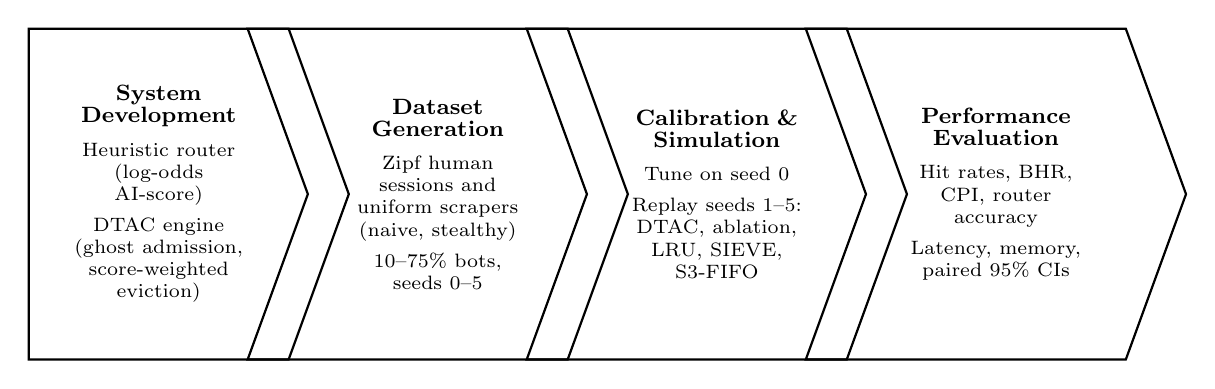
\begin{tikzpicture}[
        stage/.style={signal, signal to=east, signal from=west, draw, thick,
            signal pointer angle=140, minimum height=4.2cm, text width=2.3cm,
            align=center, font=\scriptsize, inner xsep=0.5cm}]
        \node[stage, signal from=nowhere] (dev) {
            {\footnotesize\bfseries System\\Development}\\[0.5em]
            Heuristic router\\(log-odds AI-score)\\[0.4em]
            DTAC engine\\(ghost admission,\\score-weighted\\eviction)};
        \node[stage, right=-0.55cm of dev] (gen) {
            {\footnotesize\bfseries Dataset\\Generation}\\[0.5em]
            Zipf human\\sessions and\\uniform scrapers\\(naive, stealthy)\\[0.4em]
            10--75\% bots,\\seeds 0--5};
        \node[stage, right=-0.55cm of gen] (sim) {
            {\footnotesize\bfseries Calibration \&\\Simulation}\\[0.5em]
            Tune on seed 0\\[0.4em]
            Replay seeds 1--5:\\DTAC, ablation,\\LRU, SIEVE,\\S3-FIFO};
        \node[stage, right=-0.55cm of sim] (eval) {
            {\footnotesize\bfseries Performance\\Evaluation}\\[0.5em]
            Hit rates, BHR,\\CPI, router\\accuracy\\[0.4em]
            Latency, memory,\\paired 95\% CIs};
    \end{tikzpicture}
    \caption{Methodology}

    \label{fig:methodology}
\end{figure}

This study employs an experimental systems research design structured around a proxy-cache pipeline. As illustrated in Figure~\ref{fig:methodology}, the methodology is organized into four sequential stages: System Development, Dataset Generation, Calibration and Simulation, and Performance Evaluation. First, the Heuristic Scoring Engine and the DTAC cache engine are built. Next, synthetic web logs are generated by mixing Zipf-distributed human browsing sessions with uniformly distributed AI scraper requests. The tunable constants of both components are then calibrated on a held-out log that is never used for evaluation. During simulation, the evaluation logs are replayed through DTAC, an ablated version of DTAC that ignores the AI-score, a standard LRU baseline, and two modern scan-resistant baselines (SIEVE and S3-FIFO). Finally, the performance evaluation extracts and compares hit rates, cache pollution, latency and memory metrics, with confidence intervals computed over five independently generated workloads.

\subsection{Architectural Components}
\begin{figure}[htbp]
    \centering
    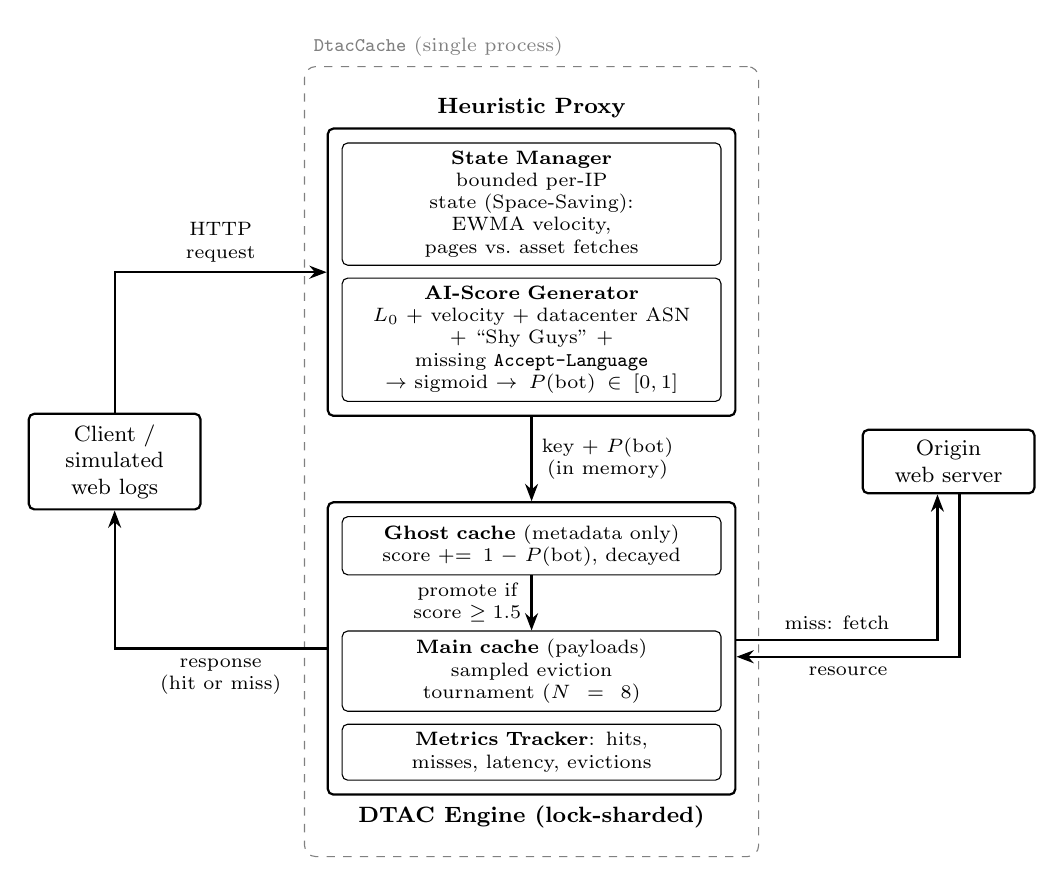
\begin{tikzpicture}[
        font=\footnotesize,
        box/.style={draw, thick, rounded corners=2pt, align=center, inner sep=4pt},
        inner/.style={draw, rounded corners=2pt, align=center, font=\scriptsize, text width=4.6cm, inner sep=3pt},
        flow/.style={-{Stealth[length=2.2mm]}, thick},
        lbl/.style={font=\scriptsize, align=center}]
        % Heuristic Proxy
        \node[inner] (state) {\textbf{State Manager}\\bounded per-IP state (Space-Saving):\\EWMA velocity, pages vs.\ asset fetches};
        \node[inner, below=0.15cm of state] (score) {\textbf{AI-Score Generator}\\$L_0$ + velocity + datacenter ASN\\+ ``Shy Guys'' + missing \texttt{Accept-Language}\\$\rightarrow$ sigmoid $\rightarrow P(\text{bot}) \in [0,1]$};
        \node[box, fit=(state)(score), inner sep=5pt, label={[font=\footnotesize\bfseries]above:Heuristic Proxy}] (router) {};
        % DTAC engine
        \node[inner, below=1.45cm of score] (ghost) {\textbf{Ghost cache} (metadata only)\\score $\mathrel{+}= 1 - P(\text{bot})$, decayed};
        \node[inner, below=0.7cm of ghost] (main) {\textbf{Main cache} (payloads)\\sampled eviction tournament ($N = 8$)};
        \draw[flow] (ghost) -- node[lbl, left] {promote if\\score $\geq 1.5$} (main);
        \node[inner, below=0.15cm of main] (metrics) {\textbf{Metrics Tracker}: hits, misses, latency, evictions};
        \node[box, fit=(ghost)(main)(metrics), inner sep=5pt, label={[font=\footnotesize\bfseries]below:DTAC Engine (lock-sharded)}] (engine) {};
        \draw[flow] (router.south) -- node[lbl, right] {key + $P(\text{bot})$\\(in memory)} (engine.north);
        % Process boundary
        \begin{scope}[on background layer]
            \node[draw, dashed, gray, rounded corners=4pt, fit=(router)(engine), inner xsep=8pt, inner ysep=22pt] (proc) {};
        \end{scope}
        \node[font=\scriptsize, gray, anchor=south west] at (proc.north west) {\texttt{DtacCache} (single process)};
        % External parties
        \node[box, text width=1.9cm, left=1.3cm of proc] (client) {Client /\\simulated\\web logs};
        \node[box, text width=1.9cm, right=1.3cm of proc] (origin) {Origin\\web server};
        \draw[flow] (client.north) |- node[lbl, above, pos=0.75] {HTTP\\request} (router.west);
        \draw[flow] (engine.west) -| node[lbl, below, pos=0.25] {response\\(hit or miss)} (client.south);
        \draw[flow] ([yshift=3pt]engine.east) -| node[lbl, above, pos=0.25] {miss: fetch} ([xshift=-4pt]origin.south);
        \draw[flow] ([xshift=4pt]origin.south) |- node[lbl, below, pos=0.75] {resource} ([yshift=-3pt]engine.east);
    \end{tikzpicture}
    \caption{System Architecture}

    \label{fig:architecture}
\end{figure}

The core of the system relies on a two-stage architectural model positioned between the incoming traffic and the origin web server, as depicted in Figure~\ref{fig:architecture}. Both stages run inside a single process: a \texttt{DtacCache} object owns the router and the cache engine and passes the computed score from one to the other in memory. The system is composed of the following primary components:

\begin{itemize}
    \item \textbf{The Heuristic Proxy (``The Brains''):} This component inspects each incoming request and serves as the analytical engine. It is subdivided into two distinct modules:
    \begin{itemize}
        \item \textit{State Manager:} This module keeps bounded per-IP state across requests: a decayed request-velocity counter and a record of how many pages an IP has fetched and whether it has ever fetched an auxiliary asset (such as \texttt{favicon.ico}, stylesheets or scripts) that a real browser would typically request.
        \item \textit{AI-Score Generator:} Utilizing the data from the State Manager together with the request's own headers and source network, this module calculates a continuous probability score ranging from 0.0 to 1.0 that quantifies how likely the request is to have originated from an automated scraper.
    \end{itemize}
    \item \textbf{The DTAC Cache:} Positioned directly upstream of the origin server, this caching engine receives the requested resource key together with the AI-score. It consists of:
    \begin{itemize}
        \item \textit{DTAC Engine (Score-Aware Cache):} The core memory management engine. Instead of a recency-ordered LRU list, it combines a metadata-only ghost cache for admission, a time-decayed popularity score per resource to which each request contributes in proportion to how human it appears, and a randomized sampling tournament for eviction. Content requested mainly by probable bots therefore accumulates little score, is rarely admitted, and is evicted first.
        \item \textit{Metrics Tracker:} An integrated monitoring component that records hits, misses, per-phase latencies and eviction events, and exports them for the Performance Evaluation phase.
    \end{itemize}
\end{itemize}

\subsection{Data Flow and Request Lifecycle}
The lifecycle of an individual request follows a unidirectional path through the architecture (see Figure~\ref{fig:architecture}):

\begin{enumerate}
    \item \textbf{Ingestion:} An HTTP request, either replayed from the simulated web logs or received by the standalone reverse proxy, arrives at the Heuristic Proxy.
    \item \textbf{Scoring and Forwarding:} The State Manager and AI-Score Generator evaluate the request and compute its 0.0--1.0 bot probability. The score is passed directly, in memory, to the DTAC engine together with the resource key. (The standalone proxy can optionally echo the score back to the client in an \texttt{X-Bot-Probability} header for debugging and benchmarking.)
    \item \textbf{Cache Evaluation:}
    \begin{itemize}
        \item \textit{Cache Hit:} If the DTAC engine already holds the requested resource in its main cache, the resource's score is updated and the cached payload is returned without contacting the origin server.
        \item \textit{Cache Miss:} If the resource is not in the main cache, its metadata is recorded (or updated) in the ghost cache and the request is forwarded to the Origin Web Server.
    \end{itemize}
    \item \textbf{Retrieval and Admission:} The origin returns the resource to the client. The payload is stored in the main cache only once the resource's accumulated, AI-score-weighted popularity crosses a promotion threshold, which in practice means a second request from a probable human. If the main cache is full, a randomized eviction tournament first removes the lowest-scoring resident entry. The origin fetch is performed outside the cache's internal locks, so a slow origin does not block unrelated requests.
\end{enumerate}

\section{Development Environment and Tools}
To ensure the reproducibility of the study, the hardware and software environments were explicitly defined and recorded alongside every experimental run.

\subsection{Hardware Specifications}
All development, testing and benchmarking was carried out on a single consumer laptop featuring a 12th Gen Intel\textsuperscript{\textregistered} Core\textsuperscript{\texttrademark} i5-1235U processor (10 cores: 2 performance and 8 efficiency cores), 16 GB of RAM, and a Solid State Drive (SSD), running Arch Linux.

The same machine was used for the initial coding, functional acceptance testing and algorithm debugging (Phase 1) and for the final workload simulations (Phase 2). To limit the influence of background processes and thermal effects on the measurements, the benchmark runs were executed strictly one at a time rather than in parallel, every reported metric is averaged over five independent workloads, and the comparisons between algorithms are made on identical request sequences (Section 3.6). Cache-efficiency metrics such as hit rates are deterministic functions of the request sequence and the algorithm, and are therefore unaffected by the hardware; only the absolute latency figures depend on it.

\subsection{Software Stack and Programming Language}
The Heuristic Proxy and the Dynamic Traffic-Aware Cache (DTAC) were developed entirely in Rust (stable toolchain, version 1.97). Rust was explicitly selected for this architecture because it bridges the gap between high-level safety and low-level system performance.

\begin{itemize}
    \item \textbf{Memory Safety:} In traditional low-level languages like C and C++, developers have direct control over memory, which allows for exceptional speed but introduces vulnerabilities such as dangling pointers, memory leaks, and buffer overflows. Rust eliminates these bugs at compile time through its strict ``ownership'' and ``borrowing'' rules, guaranteeing memory safety without relying on a runtime garbage collector.
    \item \textbf{High Performance:} Because it compiles directly to machine code and lacks the overhead of garbage collection pauses, Rust achieves low-latency execution speeds comparable to C and C++. This is critical for building a network proxy and cache, where computing the AI-score must not introduce latency that outweighs the time saved by caching.
    \item \textbf{Concurrency:} Rust's type system prevents data races in multi-threaded environments, enabling ``fearless concurrency'' when processing simultaneous HTTP requests.
\end{itemize}

The cache engine is built from the standard library's \texttt{HashMap} and \texttt{Vec} types: each lock shard keeps a hash map from resource key to an index into a dense vector of entries, so that a uniformly random entry can be sampled and removed in constant time (by swapping it with the last element). The State Manager's bounded per-IP table uses a \texttt{HashMap} paired with ordered \texttt{BTreeSet} indices. The asynchronous runtime \texttt{tokio} handles concurrent request processing; the standalone reverse proxy is built on the \texttt{axum} web framework and forwards misses with the \texttt{reqwest} HTTP client. Latencies are recorded into \texttt{hdrhistogram} histograms, and operational metrics are exported through OpenTelemetry to a Prometheus endpoint.

\subsection{Simulation and Log Replay Tools}
Because testing against a live production server introduces unpredictable variables, the workloads were completely simulated. Dedicated tools were developed for data generation, log replay and experiment orchestration:

\begin{itemize}
    \item \textbf{Data Generator (\texttt{generate\_logs.py}):} A Python script (using \texttt{numpy}) that outputs synthetic HTTP request logs in newline-delimited JSON. It blends Zipf-distributed human browsing sessions with uniformly scanning bot traffic at a chosen bot ratio. Each record carries its timestamp, client IP, path, headers, object size and a ground-truth label (human or bot), and the same random seed always produces byte-identical files.
    \item \textbf{Log Replayer (\texttt{replay\_bench}):} A Rust binary that loads a log into memory and replays every record against the chosen cache algorithm \emph{in-process}, with a bounded number of requests in flight concurrently. All time-dependent logic (velocity, score decay) reads a simulated clock that is set to each record's logged timestamp, so the replay can run far faster than real time while the algorithms still observe the log's original timeline. Running in-process removes network variance, so the measured differences reflect cache behaviour rather than the network stack.
    \item \textbf{Networked Validation (\texttt{dtac\_standalone} and \texttt{origin\_stub}):} The replayer can alternatively send every record as a real HTTP request over \texttt{localhost} to the standalone DTAC reverse proxy, which forwards misses to a stub origin server that returns the requested number of bytes. This mode was used to confirm that the in-process results match the behaviour of the full networked system.
    \item \textbf{Experiment Harness (\texttt{run\_experiments.py}):} A Python script that performs the calibration sweeps, generates each seed's logs, runs every cell of the experiment grid sequentially, and aggregates the results into means, confidence intervals and paired differences.
\end{itemize}

\section{System Implementation}
This section details the algorithmic design and software engineering required to translate theoretical bot detection into a high-performance, deployable network component. The system is divided into two interconnected components: a Heuristic Proxy that evaluates incoming traffic via bounded-memory Log-Odds classification, and a Dynamic Traffic-Aware Cache (DTAC) that leverages randomized eviction, a metadata-only ghost cache, and resource-specific time-decayed scoring to limit automated cache pollution. Every per-request operation in both components has a small, bounded cost that does not grow with the volume of traffic observed: the router's state updates take $\mathcal{O}(\log K)$ time for a fixed tracking capacity $K$, and the cache engine's lookups take constant time with evictions costing $\mathcal{O}(N)$ for a small, fixed sample size $N$.

\subsection{The Heuristic Proxy and AI-Score Generator}
The Heuristic Proxy acts as the initial ingress point for all network traffic. Its primary function is to classify incoming HTTP requests probabilistically without relying on heavy client-side challenges. To keep the scoring cost to microseconds, this was implemented through a Composite Trust Scoring architecture relying on a continuous Log-Odds model rather than rigid binary thresholds \cite{chandra_composite_2026}.

\textbf{The Bounded-Memory State Manager:}
To evaluate behavioral anomalies across a session without succumbing to memory exhaustion from internet-scale traffic, the proxy does not use an unbounded \texttt{HashMap} keyed by IP address. Instead, the State Manager implements the Space-Saving algorithm \cite{metwally_efficient_2005} to address the ``Top-K Elephant Flow'' problem commonly encountered in network measurement (Gong et al., 2018). By utilizing a Rust \texttt{HashMap} paired with ordered \texttt{BTreeSet} indices, the proxy maintains strict bounds on memory ($\mathcal{O}(K)$ space for a fixed capacity of $K$ tracked IPs, with $\mathcal{O}(\log K)$ updates). When the table is full, the IP with the smallest count is replaced and its count is inherited by the newcomer, as the algorithm prescribes. Counts decay with a configurable half-life (one hour), so the structure tends to retain persistent high-volume clients (``elephant flows'') while low-volume visitors (``mice flows'') are naturally displaced.

Within this bounded state, the proxy tracks request velocity using an Exponentially Weighted Moving Average (EWMA). Because human request inter-arrival times naturally follow heavy-tailed distributions characterized by micro-bursts \cite{li_queuing_2018}, the proxy maintains an instantaneous velocity score $v$ using a time-decayed counter rather than storing arrays of timestamps. The counter is a fixed-point integer scaled by 1024; on each request it is halved, via a base-2 bitwise right shift, once for every elapsed velocity tick (5 seconds after calibration) and then incremented by one request. After ten idle ticks the counter is reset. This accommodates natural human burstiness while penalizing sustained automated scraping at a constant cost per request.

\textbf{The AI-Score Generation (Log-Odds Classification):}
Instead of a rudimentary weighted sum, the proxy calculates an aggregate score in the Log-Odds domain, in the style of a Naive Bayes classifier. This allows the proxy to begin with a baseline prior probability of automated traffic and perform efficient additive arithmetic. The prior log-odds $L_0$ is derived from an explicit assumed bot base rate $p_0$:

\begin{equation}
L_0 = \ln\left(\frac{p_0}{1 - p_0}\right)
\end{equation}

With the calibrated $p_0 = 0.02$, $L_0 \approx -3.89$: every request is assumed human until the evidence says otherwise, and a clean human request scores a bot probability of about 0.02.

For every triggered heuristic $i$, a weight $W_i$ is added to the running log-odds score. In an idealized Naive Bayes model this weight would be the log-likelihood ratio of observing the evidence $E_i$ from a bot versus a human:

\begin{equation}
W_i = \ln\left(\frac{P(E_i \mid \text{Bot})}{P(E_i \mid \text{Human})}\right)
\label{eq:llr}
\end{equation}

Estimating these ratios requires labelled real-world traffic, which was not available to this study. Estimating them from the synthetic workload instead would be circular, because the workload generator was written to trigger exactly these heuristics (Section 3.4.3). The weights used were therefore \emph{calibrated} on a held-out workload to maximize the separation between human and bot scores under a false-positive constraint, and Equation~\ref{eq:llr} serves as the motivation for the additive model rather than as the method for obtaining its weights.

The heuristic evaluation engine processes four independent signals:
\begin{itemize}
    \item \textbf{Passive Structural Anomalies (``Shy Guys''):} Following \citeA{van_boxem_shy_2026}, the proxy penalizes IPs that fetch pages but never fetch auxiliary assets (favicon, stylesheets, scripts, images or fonts). Browsers request such assets once and then cache them, so the signal is that an IP has \emph{never} fetched one, not that it skipped one on its last page. A grace period of 12 page requests prevents short human visits from being flagged. The heuristic adds $W_{fav} = 2$.
    \item \textbf{Header Anomalies:} Requests that lack an \texttt{Accept-Language} header, which every mainstream browser sends, receive $W_{hdr} = 4$. Other header checks (such as \texttt{Sec-CH-UA} consistency or header ordering) were not implemented.
    \item \textbf{Infrastructure Origin:} The client IP is looked up in an offline copy of the public iptoasn \texttt{ip2asn} database, which maps IP ranges to Autonomous System Numbers (ASNs), using binary search over the sorted ranges ($\mathcal{O}(\log n)$). If the ASN belongs to a curated list of cloud and hosting providers, the request receives $W_{asn} = 3$, reflecting the established use of datacenter origin as a baseline filter in automated traffic detection \cite{martinez_llamas_balancing_2025}.
    \item \textbf{Graded Request Velocity:} Rather than applying a binary step-function \cite{duskin_distinguishing_2009}, the tracked EWMA velocity $v$ applies a continuously scaling penalty inspired by the Weber-Fechner Law. Once a baseline human burst threshold $v_{\tau}$ is exceeded, a graded log-weight is applied:
\end{itemize}

\begin{equation}
W_{velocity} = \max\left(0, \alpha \cdot \ln\left(\frac{v}{v_{\tau}}\right)\right)
\end{equation}

with the calibrated $v_{\tau} = 3$ (in units of the decayed per-tick counter) and $\alpha = 2$.

Once all heuristic weights are summed ($L = L_0 + \sum W_i$), the final log-odds score is converted back to a continuous probability $P(\text{bot})$ ranging from 0.0 to 1.0 using the sigmoid function:

\begin{equation}
P(\text{bot}) = \frac{1}{1 + e^{-L}}
\end{equation}

This value expresses the router's confidence that the request originated from an automated scraper and is passed directly to the DTAC engine. The router also reports which heuristics fired for each request, which allows the evaluation to measure how often each signal fires on human and on bot traffic.

Algorithm 1 illustrates the complete ingress pipeline, demonstrating how the bounded-memory Space-Saving structure and Log-Odds heuristic scoring operate for each incoming request.

\begin{verbatim}
Algorithm 1: Ingress Proxy Pipeline & Log-Odds AI-Score Generation
-------------------------------------------------------------------
Input: incoming_request
Global State:
    SpaceSaver: Bounded per-IP tracker (HashMap + BTreeSet)
    L_0: Baseline prior log-odds, ln(0.02/0.98) = -3.89
    W_asn = 3, W_fav = 2, W_hdr = 4: calibrated weights
    TICK = 5 s, BURST_THRESHOLD = 3, ALPHA = 2, SHY_PAGES = 12

1:  client_ip <- incoming_request.IP
2:  now <- clock.now()
3:
4:  // --- PHASE 1: State Retrieval & Bounded Memory Management ---
5:  // O(log K); evicts the lowest-count IP when the table is full
6:  ip_state <- SpaceSaver.get_or_add_and_evict(client_ip)
7:
8:  // --- PHASE 2: EWMA Velocity Calculation (Bitwise) ---
9:  ticks <- (now - ip_state.last_seen) / TICK
10: if ticks > 10 then
11:     new_velocity <- 1024  // Reset, plus 1 request (x1024)
12: else
13:     decayed_v <- ip_state.velocity >> ticks  // Bitwise shift
14:     new_velocity <- decayed_v + 1024
15: end if
16:
17: // Update structural history and commit state
18: if is_auxiliary_asset(incoming_request.path) then
19:     ip_state.fetched_asset <- TRUE
20: else
21:     ip_state.pages <- ip_state.pages + 1
22: end if
23: ip_state.last_seen <- now
24: ip_state.velocity <- new_velocity
25: SpaceSaver.update(client_ip, ip_state)
26:
27: // --- PHASE 3: Log-Odds Heuristic Evaluation ---
28: score <- L_0
29:
30: // Heuristic A: Continuous Graded Velocity Penalty
31: float_v <- new_velocity / 1024.0
32: if float_v > BURST_THRESHOLD then
33:     score <- score + (ALPHA * ln(float_v / BURST_THRESHOLD))
34: end if
35:
36: // Heuristic B: Infrastructure Origin (Datacenter ASN)
37: if ASN_Database.is_datacenter(client_ip) then
38:     score <- score + W_asn
39: end if
40:
41: // Heuristic C: "Shy Guys" Passive Behavioral Check
42: if ip_state.pages >= SHY_PAGES
        and not ip_state.fetched_asset then
43:     score <- score + W_fav
44: end if
45:
46: // Heuristic D: Missing Accept-Language Header
47: if incoming_request.missing_header("Accept-Language") then
48:     score <- score + W_hdr
49: end if
50:
51: // --- PHASE 4: Sigmoid Conversion & Forwarding ---
52: bot_probability <- 1.0 / (1.0 + exp(-score))
53:
54: return DTAC_Engine.access(incoming_request.path,
                           bot_probability)
\end{verbatim}

\subsection{The Dynamic Traffic-Aware Cache (DTAC) Engine}
The second component of the system is the DTAC engine, positioned upstream of the origin server. Rather than utilizing deterministic eviction algorithms (such as LRU or LFU), which either fail to account for long-term popularity or suffer from sequential scan pollution under bot traffic \cite{zhang_rethinking_2026}, the DTAC engine was implemented using a Randomized Eviction architecture combined with a resource-specific decayed popularity score and a metadata-only Ghost Cache.

\textbf{Resource-Based Decayed Score \& Lock Sharding:}
Unlike the State Manager (Section 3.4.1), which tracks the behavioral velocity of client IP addresses, the DTAC engine tracks the popularity score of the requested resources (e.g., specific URLs or assets).

Whenever a resource is requested, whether it is in the main cache or the ghost cache, its score $s$ is first decayed for the elapsed time and then incremented by $1 - P(\text{bot})$, the complement of the request's AI-score. A request from a confident human (bot probability $\approx 0.02$) adds almost a full point, whereas a highly suspicious request adds effectively zero. This increment is the mechanism that connects the router's output to caching behavior. Decay is applied lazily, only when an entry is touched, in discrete half-life steps:

\begin{equation}
s(t) = s(t_0) \cdot 2^{-\lfloor (t - t_0) / h \rfloor}
\end{equation}

where $t_0$ is the entry's last access and $h$ is the decay half-life. After 32 half-lives the score is treated as zero. With the calibrated half-life of $h = 4$ hours, which exceeds the duration of the benchmark logs, the score behaves much like a human-weighted frequency count, so the policy approaches a Least Frequently Used (LFU) ordering with recency as a tie-breaker. A shorter half-life would make the cache adapt faster when popularity shifts, at the cost of forgetting stable popularity.

Updating this resource score on every read introduces a known concurrency bottleneck: the ``read-path write penalty.'' To prevent concurrent threads from blocking one another while updating the metadata of a popular asset, the system implements lock sharding. Incoming requests are hashed by resource key to one of several independent, mutex-protected shards, each with its own share of the capacity, its own ghost cache and its own eviction. The shard count is chosen automatically as the largest power of two up to 256 that leaves at least 64 entries per shard (for example, 128 shards at a capacity of 10\,000 entries); very small shards would distort the sampling-based eviction described below.

\textbf{Cold-Start Mitigation via Metadata-Only Ghost Cache:}
To resolve the ``Cold Start'' problem, where brand new items are evicted before they can establish a popularity score, while conserving memory, DTAC implements a two-stage admission design inspired by the S3-FIFO caching model \cite{yang_fifo_2023}.

When a cache miss occurs, the system does not store the full data payload. Instead, it records only the resource's identifier, last access time and initial score inside the Ghost Cache (a lightweight, metadata-only structure), and the request is served from the origin. If the resource receives subsequent requests and its decayed score crosses a promotion threshold (calibrated to 1.5), it graduates: the payload is fetched from the origin and stored in the Main Cache. Because a clean human request contributes about 0.98, two human requests promote an item, whereas a scan of requests that each score near 1.0 never accumulates enough score to be admitted. One-off scraper requests therefore never consume main-cache memory.

The ghost cache is itself bounded, at eight times the main-cache capacity per shard. When it is full, a ghost entry is evicted with the same score-aware tournament as the main cache. Entries created by bot requests start with a score near zero and therefore lose first, so a uniform bot scan cannot push popular human items out of the ghost before their second request, as a plain FIFO ghost queue would allow.

The origin fetch for a promotion is performed after the shard lock has been released. Once the payload arrives, the lock is re-acquired and the engine re-checks whether another concurrent request has already promoted the same resource, so a slow origin never blocks other requests and a popular item is never inserted twice.

\textbf{The Eviction Tournament (The Power of N Choices):}
When the Main Cache reaches capacity, the system triggers a randomized eviction tournament instead of maintaining a globally sorted priority queue. The algorithm samples $N$ random entries from the shard (calibrated to $N = 8$), lazily calculates their currently decayed scores, and evicts the entry with the lowest score, breaking ties in favor of evicting the entry with the oldest last access. Once scores have decayed to zero, eviction therefore falls back to LRU order instead of being random. This approach mirrors modern sampling-based eviction frameworks such as Google's HALP (Google Research, 2023) and RankCache (Beckmann et al., 2018). While sampling introduces a minor statistical variance compared to sorting the entire cache, each eviction costs only $\mathcal{O}(N)$ for a small, fixed $N$, independent of cache size, and requires no global ordering to be maintained on every hit.

\begin{verbatim}
Algorithm 2: DTAC Admission, Eviction, Sharding and Ghost Cache
-------------------------------------------------------------------
Input: requested_resource, request_bot_prob (Float 0.0 to 1.0)
Parameters: N_SAMPLES = 8, PROMOTION_THRESHOLD = 1.5,
            HALF_LIFE = 4 h, GHOST_CAP = 8 x shard capacity
State per shard: MainCache (payload + metadata),
                 GhostCache (metadata only)

1:  // Phase 1: Concurrency Management (Lock Sharding)
2:  shard <- shards[hash(requested_resource) % NUM_SHARDS]
3:  acquire_lock(shard)
4:  increment <- 1.0 - request_bot_prob
5:
6:  // Phase 2: Main Cache Hit
7:  if shard.MainCache.contains(requested_resource) then
8:      meta <- shard.MainCache.metadata(requested_resource)
9:      meta.score <- decay(meta.score, now - meta.last_access)
                      + increment
10:     meta.last_access <- now
11:     payload <- shard.MainCache.payload(requested_resource)
12:     release_lock(shard)
13:     return HIT(payload)
14: end if
15:
16: // Phase 3: Miss -- update or create the ghost entry
17: if shard.GhostCache.contains(requested_resource) then
18:     g <- shard.GhostCache.metadata(requested_resource)
19:     g.score <- decay(g.score, now - g.last_access) + increment
20:     g.last_access <- now
21: else
22:     if shard.GhostCache.size() >= GHOST_CAP then
23:         evict_by_tournament(shard.GhostCache)
24:     end if
25:     g <- shard.GhostCache.insert(requested_resource, now,
                                     increment)
26: end if
27: promote <- (g.score >= PROMOTION_THRESHOLD)
28: release_lock(shard)
29:
30: // Phase 4: Origin fetch outside the lock
31: payload <- fetch_from_origin(requested_resource)
32: if promote then
33:     acquire_lock(shard)
34:     if not shard.MainCache.contains(requested_resource) then
35:         if shard.MainCache.is_full() then
36:             evict_by_tournament(shard.MainCache)
37:         end if
38:         g <- shard.GhostCache.remove(requested_resource)
39:         shard.MainCache.insert(requested_resource, payload, g)
40:     end if  // else: a concurrent request already promoted it
41:     release_lock(shard)
42: end if
43: return MISS(payload)
44:
45: // --- Helper: stepwise half-life decay ---
46: function decay(score, delta_t):
47:     k <- floor(delta_t / HALF_LIFE)
48:     if k >= 32 then return 0
49:     return score / 2^k
50:
51: // --- Helper: Eviction Tournament ---
52: function evict_by_tournament(store):
53:     candidates <- store.random_samples(N_SAMPLES)
54:     victim <- argmin over candidates of
55:           (decay(c.score, now - c.last_access), c.last_access)
56:     store.swap_remove(victim)  // O(1) removal from dense vector
\end{verbatim}

\subsection{Tuning Parameters and System Calibration}
The efficacy of both the Heuristic Proxy and the DTAC engine relies heavily on the calibration of their numerical thresholds. Because internet traffic follows heavy-tailed Zipfian distributions \cite{breslau_web_1999}, poorly chosen values lead either to excessive false positives (penalizing humans) or to cache pollution. The system's parameters must therefore be tuned empirically against the target network's traffic. In this study every constant is exposed through JSON configuration rather than hard-coded, and all of them were calibrated on a dedicated tuning workload (seed 0) that is never used in the reported evaluation (seeds 1--5).

The configuration is governed by three primary categories.

\textbf{1. Velocity and Bounded-Memory Thresholds (State Manager and Engine)}
The parameters governing the EWMA velocity counter, the score decay, and the ghost cache dictate the proxy's sensitivity to automated scrapers and the engine's memory of popularity.
\begin{itemize}
    \item \textbf{Velocity Tick and Human Burst Threshold ($v_{\tau}$):} The velocity counter is halved once per tick, and the threshold is the decayed counter value below which no penalty is applied. Initial values of a 1-second tick and $v_{\tau} = 10$ never flagged the naive bots in the benchmark (whose counters settled near 7). After calibration, a 5-second tick with $v_{\tau} = 3$ flags nearly all naive bots, at the cost of the velocity heuristic also firing on about 4\% of human requests from fast multi-page sessions, never enough on its own to push a human above a bot probability of 0.5.
    \item \textbf{Velocity Scaling Factor ($\alpha$):} Determines the aggressiveness of the continuous Log-Odds penalty once an IP exceeds $v_{\tau}$. It was kept at $\alpha = 2$ and not swept.
    \item \textbf{Score Decay Half-Life ($h$):} The initial half-life of one second made scores vanish between two page views of the same session, so the main cache stayed almost empty (25--130 of its 10\,000 slots). Human hit rate rose with every increase of the half-life up to the largest value tested, 4 hours.
    \item \textbf{Ghost Cache Promotion Threshold:} The decayed score a resource must accumulate in the metadata-only Ghost Cache before its payload is admitted. The calibrated value of $1.5$ means ``promote on the second human request''. A threshold of $0.5$ (admit on the first human request) performed worse at a capacity of 10\,000 entries because one-off human requests then competed with popular items.
    \item \textbf{Ghost Cache Capacity:} Eight times the main-cache capacity; any multiplier of 2 or more improved human hit rate by about 1.5 points over a ghost the same size as the main cache.
\end{itemize}

\textbf{2. Probabilistic Heuristic Weights (Log-Odds Engine)}
\begin{itemize}
    \item \textbf{Prior Probability ($L_0$):} The baseline assumption of automated traffic, expressed through the assumed bot base rate $p_0$. For a heavily targeted public API where 60\% of traffic is automated, the prior log-odds would be $L_0 = \ln(0.60 / 0.40) = +0.405$. Calibration favored the low prior $p_0 = 0.02$ ($L_0 \approx -3.89$), because it lets a clean human request contribute almost a full point ($0.98$) to a resource's score. Higher priors (0.3) pushed returning human visitors above a bot probability of 0.5 once a single heuristic fired.
    \item \textbf{Evidence Weights ($W_i$):} As discussed in Section 3.4.1, these were chosen to maximize the gap between the mean bot probability of bots and that of humans, subject to keeping the false-positive rate for returning human visitors at or below 5\%. The calibrated weights ($W_{hdr} = 4$, $W_{asn} = 3$, $W_{fav} = 2$) are much smaller than the empirical log-likelihood ratios measured on the synthetic data (up to $+12$), because a sum of such large terms would saturate every bot at 1.0 and the weights would stop mattering. If a network naturally serves a high volume of enterprise VPN users, the weight for the datacenter heuristic should be decreased to limit false positives.
\end{itemize}

\textbf{3. Eviction Tournament Sample Size ($N$)}
An important parameter in the DTAC engine is $N$, the number of random items sampled during an eviction tournament. If $N$ is too small, the system risks evicting a highly popular item. If $N$ is too large, the engine wastes CPU cycles evaluating decayed scores, defeating the purpose of randomized eviction.

To reason about a suitable $N$, the framework of Order Statistics can be used to evaluate the expected value of the minimum, $E[X_{(1)}]$. In a cache, the distribution of item scores is typically bimodal: a large cluster of low-scoring ``junk'' items (decayed or one-off requests) and a smaller cluster of high-scoring popular items. This can be modeled as a Gaussian Mixture Model (GMM).

While there is no clean algebraic formula for the exact expected minimum of a GMM, the ``sweet spot'' for $N$ can be determined logically. As $N$ increases, the expected minimum drops sharply at first but then hits a point of extreme diminishing returns. This occurs because once the algorithm draws at least one sample from the ``lower mode'' (the junk items), the minimum is effectively bounded by that lower distribution.

Therefore, selecting $N$ is a function of confidence. Let $p$ be the proportion of the cache population that belongs to the lower distribution (evictable items). The probability of failing to pick from this lower distribution in $n$ tries is $(1-p)^n$. The probability $P$ of successfully sampling the lower distribution at least once is:

\begin{equation}
P = 1 - (1-p)^n
\end{equation}

To find an $N$ that achieves a specific confidence level, we solve for $n$:

\begin{equation}
n = \frac{\ln(1 - P)}{\ln(1 - p)}
\end{equation}

\textit{Estimating $N$:} Suppose the cache is heavily utilized, and only 20\% of the cache consists of evictable junk items ($p = 0.20$). To be 95\% confident ($P = 0.95$) that the random sample includes at least one of these candidates, the required sample size is:

\begin{equation}
n = \frac{\ln(1 - 0.95)}{\ln(1 - 0.20)} = \frac{\ln(0.05)}{\ln(0.80)} = \frac{-2.995}{-0.223} \approx 13.4
\end{equation}

Under this assumption, $N = 14$ would give a 95\% probability of finding a highly decayed item without the cost of sorting the entire cache.

For environments where the cache churn is higher and junk items make up a larger proportion of the cache (e.g., $p = 0.50$), the required sample size drops drastically. Achieving 95\% confidence in this scenario requires only $N = 5$ ($1 - 0.5^5 = 0.968$). This aligns with the default parameters established by industry implementations; Redis utilizes $N = 5$ for its \texttt{allkeys-lfu} policy as a balance between CPU efficiency and eviction accuracy (Redis Core Architecture).

The analysis therefore bounds the useful range of $N$ to roughly 5--14. Empirical calibration within this range selected $N = 8$: it was consistently better than $N = 5$, while $N = 14$ was within 0.03 percentage points of it on the tuning workload, confirming the diminishing returns predicted above.

\textbf{Calibration Procedure:}
The constants were calibrated by coordinate descent on the tuning seed, on the naive workload (Section 3.5) at 30\% and 75\% bot traffic and a cache capacity of 10\,000 entries. Each group of parameters was swept on a coarse grid with all others held fixed, followed by a refinement around the chosen value; a new value replaced the current one only if it improved the objective by more than a small tolerance. The router was calibrated first, maximizing the class-mean gap (the mean bot probability of bot requests minus that of human requests) subject to a returning-visitor false-positive rate of at most 5\%. The engine was then calibrated with the router fixed, maximizing human hit rate. Table~\ref{tab:calibration} lists the resulting values. The constants were not re-tuned for other cache capacities; a check at the other capacities found that at 20\,000 entries a promotion threshold of 0.5 would have performed about 2.3 percentage points better than the calibrated 1.5.

\begin{table}[htbp]
    \centering
    \caption{Initial and calibrated values of the router and engine constants}
    \label{tab:calibration}
    \begin{tabular}{llll}
        \toprule
        Parameter & Component & Initial & Calibrated \\
        \midrule
        Prior bot rate $p_0$ & Router & 0.1 & 0.02 \\
        $W_{asn}$ / $W_{fav}$ / $W_{hdr}$ & Router & 1.5 / 1.2 / 1.0 & 3 / 2 / 4 \\
        Velocity tick / $v_{\tau}$ & Router & 1 s / 10 & 5 s / 3 \\
        Shy Guys page threshold & Router & 5 & 12 \\
        Score half-life $h$ & Engine & 1 s & 4 h \\
        Promotion threshold & Engine & 2.0 & 1.5 \\
        Sample size $N$ & Engine & 5 & 8 \\
        Ghost capacity multiplier & Engine & 4 & 8 \\
        \bottomrule
    \end{tabular}
\end{table}

\section{Workload Simulation and Data Generation}
Testing caching algorithms against a live production server introduces uncontrolled variables (such as network latency spikes, hardware throttling, and unpredictable user behavior) that make precise metric evaluation nearly impossible, and labelled production traffic with ground truth about which requests come from bots was not available. To ensure that the performance of the DTAC algorithm was accurately and reproducibly measured, synthetic workloads were generated with the Python data generator (Section 3.3.3). Every log is fully determined by its random seed; five evaluation seeds (1--5) and one tuning seed (0) were generated.

\subsection{Simulating Legitimate Human Traffic}
Human web browsing naturally exhibits temporal locality and highly skewed popularity patterns, heavily favoring a small subset of ``hot'' web pages. To simulate this behavior, the data generator draws the pages that humans request from a Zipfian distribution \cite{breslau_web_1999}.

In a Zipfian distribution, the probability $P(k)$ of a request for the $k$-th most popular web object out of a total catalog size of $N$ items is defined as:

\begin{equation}
P(k) = \frac{1/k^\alpha}{\sum_{n=1}^{N} (1/n^\alpha)}
\end{equation}

For the simulation, the catalog size ($N$) was established at 100,000 unique web objects. The skewness parameter ($\alpha$), which dictates the intensity of the popularity concentration, was set to 0.8, a standard baseline for mirroring realistic human web traffic. Every object has a fixed size drawn once from a lognormal distribution with a median of 16 KB, clipped to the range 512 B--2 MB, so byte-level metrics can be computed.

Human traffic is generated as browser \emph{sessions} rather than as independent requests. Sessions arrive as a Poisson process; each session uses a single IP address, views a geometrically distributed number of pages (mean 5) drawn from the Zipf catalog, and waits an exponentially distributed think time (mean 8 seconds) between pages. Session arrivals are frequent enough to keep the aggregate human rate at about 12.5 requests per second. Every request carries standard browser headers, including a browser \texttt{User-Agent} and \texttt{Accept-Language}. Seventy percent of sessions are \emph{new visitors}, who fetch \texttt{/favicon.ico} once after their first page; the remaining 30\% are \emph{returning visitors}, who already have the favicon cached and never fetch it. Returning visitors who view 12 or more pages are therefore realistic false positives for the ``Shy Guys'' heuristic, which allows the evaluation to measure its cost to humans. Human IP addresses never fall in datacenter ranges.

Crucially, for a given seed the generator produces a single human request stream that is reused, unchanged, in every bot-ratio file and in both bot workloads. Differences in human hit rate across bot ratios and across algorithms are therefore caused by the bots and the algorithms alone.

\subsection{Simulating AI Scraper Traffic}
Conversely, automated AI scrapers and LLM data harvesters utilize ``scan'' patterns characterized by high-volume, single-use access over broad swaths of a website \cite{zhang_rethinking_2026}. To simulate this, bot requests are drawn from a uniform distribution over the \emph{entire} catalog, overlapping with the pages humans request. In a uniform distribution, the probability of requesting any specific item is equal, resulting in very little temporal recurrence and effectively mimicking the one-hit-wonder behavior of scrapers. Two bot workloads were generated.

\textbf{Naive scrapers} are imbued with the mechanical signatures the Heuristic Proxy is designed to detect:
\begin{itemize}
    \item They never request auxiliary assets such as \texttt{favicon.ico}.
    \item They omit browser headers, including \texttt{Accept-Language} and \texttt{Sec-CH-UA}.
    \item Each bot IP sends at a steady, mechanical rate of 3.6 requests per second ($\pm$5\% jitter), in 30-second on/off cycles. The pool of IPs grows with the bot ratio, so that each IP's rate is the same at every ratio and only the number of IPs changes.
    \item About 64\% of bot IPs fall in IP ranges that the ASN fixture used for the benchmark maps to datacenter providers; the rest use reserved documentation (TEST-NET) addresses that match no ASN.
\end{itemize}

The ASN fixture shipped with the implementation was written to cover the generator's datacenter bot ranges, so the datacenter signal is correct by construction in this benchmark. It demonstrates that the lookup works and how much a correct ASN signal helps the cache, not that ASN detection works on real traffic.

\textbf{Stealthy scrapers} imitate browser sessions in order to evaluate where the heuristics stop working. They send full browser headers (including \texttt{Accept-Language}, \texttt{Sec-CH-UA} and a human \texttt{User-Agent}) from fresh, residential-looking IP addresses, issue only about 5 requests per IP with exponential think times, and fetch \texttt{/favicon.ico} once per IP, which defeats the ``Shy Guys'' heuristic. They still scan the catalog uniformly and therefore still pollute the cache.

\subsection{Traffic Mixing and Ratios}
To evaluate the DTAC system under varying levels of infrastructure strain, the generator blends the human sessions and the bot traffic into chronological, single-stream request logs. For a target bot ratio $r$ and $H \approx 100{,}000$ human measurement requests, a file contains $B = H \cdot r / (1 - r)$ bot requests spread evenly over the entire measurement window, so that the bot share is approximately $r$ throughout the timeline rather than concentrated at the start.

The traffic was multiplexed to create multiple distinct datasets, each representing a different severity of AI interference. The test ratios were defined by the percentage of total traffic originating from simulated scrapers:
\begin{itemize}
    \item \textbf{10\% Bot Traffic:} Representing a baseline, low-threat environment.
    \item \textbf{30\% Bot Traffic:} Representing moderate, localized scraper activity.
    \item \textbf{50\% Bot Traffic:} Representing a heavy data-harvesting event.
    \item \textbf{75\% Bot Traffic:} Representing a severe scan event capable of inducing cache thrashing \cite{zhang_rethinking_2026}.
\end{itemize}

Each log is prefixed with a warm-up phase of about 50,000 purely human requests (Section 3.6.1). For every seed, this yields eight files (two bot workloads at four ratios). Alongside each file the generator writes a metadata file recording the seed, every generator parameter and the generator's version, which the replayer copies into its results.

\section{Experimental Setup and Benchmarking Procedures}
To empirically validate the efficacy of the DTAC algorithm against standard and state-of-the-art caching mechanisms, a controlled benchmarking protocol was established and executed on the laptop described in Section 3.3.1.

\subsection{The Benchmarking Protocol}
The lifecycle of each individual experiment followed a three-step protocol to ensure that the collected data reflected steady-state behavior rather than artificial testing anomalies.

\begin{enumerate}
    \item \textbf{Step 1: Cache Warm-Up:} A cache starting from an empty state (a ``cold'' cache) naturally experiences an initial 100\% miss rate as it begins storing objects, which skews performance metrics. Therefore, before any simulated scraper traffic, each log begins with a fixed prefix of about 50,000 purely human requests. These requests are processed by the cache exactly like any other request, so the cache is populated, but they are excluded from every reported metric and timing.
    \item \textbf{Step 2: Mixed Traffic Replay:} Immediately after the warm-up, the replayer continues with the measurement phase, in which human and bot requests are interleaved at the file's bot ratio. Each combination of seed, workload, bot ratio, algorithm and capacity was run as a separate replay, and the replays were executed sequentially so that runs never competed for CPU.
    \item \textbf{Step 3: Metric Logging:} Throughout the measurement phase, the replayer recorded the outcome of every request (hit or miss, bytes served, latency of each phase, and the router's score), sampled the contents of the cache periodically to measure pollution, and recorded every main-cache eviction together with the label (human or bot) of the request that had caused the evicted entry to be admitted. Each run wrote all of its metrics, its configuration and the software version to a JSON file.
\end{enumerate}

The experiment grid comprised five seeds (1--5), two bot workloads (naive and stealthy), four bot ratios (10\%, 30\%, 50\% and 75\%) and five algorithms at a primary cache capacity of 10\,000 entries (10\% of the catalog). In addition, a capacity sweep at 1\,000, 5\,000, 10\,000 and 20\,000 entries (1--20\% of the catalog) was run for the naive workload at 30\% and 75\% bot traffic. In total the grid contained 350 replays. A single replay was also repeated over the network (Section 3.3.3) to validate the in-process results.

\subsection{Baseline Comparison}
To isolate and quantify the performance impact of the AI-aware design, every workload was replayed through five algorithms:

\begin{itemize}
    \item \textbf{Standard LRU (Control):} A sharded Least Recently Used cache that ignores the AI-score entirely and treats all incoming traffic (both human and bot) with equal temporal importance. This establishes how severely a standard cache degrades under scan patterns.
    \item \textbf{SIEVE and S3-FIFO (State-of-the-art baselines):} The two modern scan-resistant algorithms reviewed in Chapter 2 \cite{zhang_sieve_2024, yang_fifo_2023}, implemented for this study. They are also blind to the AI-score and infer the value of objects from access patterns alone.
    \item \textbf{DTAC without the score (Ablation):} The DTAC engine with every request assigned the same score a clean human request would receive ($\text{sigmoid}(L_0) = 0.02$), so bots cannot be told apart from humans. Using this constant, rather than zero, keeps the promotion speed identical to DTAC's for human traffic. Comparing DTAC with this ablation separates the contribution of the AI-score from that of the ghost cache and the decayed-score tournament.
    \item \textbf{DTAC (Experimental):} The full system, in which the router's AI-score weights every request's contribution to admission and eviction.
\end{itemize}

All five algorithms share the same shard count and the same per-shard capacity split, so only the caching policy differs between them. Because the request sequence, the total cache capacity and the hardware were identical across the five runs of a given cell, any divergence in the final performance metrics can be attributed to the algorithms themselves.

\subsection{Statistical Analysis}
Each metric is reported as the mean over the five evaluation seeds with a 95\% confidence interval computed from the $t$-distribution ($n = 5$). Because every algorithm processes exactly the same human requests for a given seed, comparisons between DTAC and each alternative are made as \emph{paired differences}: the difference $\text{metric}(\text{DTAC}) - \text{metric}(X)$ is computed separately for each seed, and the mean and 95\% confidence interval of these differences are reported. A difference whose confidence interval excludes zero is treated as statistically significant; one whose interval includes zero is reported as a tie. This paired design is considerably more sensitive than comparing two overlapping confidence intervals.

\section{Evaluation Metrics}
To evaluate the Dynamic Traffic-Aware Caching (DTAC) algorithm against the baselines, the benchmarking protocol recorded a specific set of quantitative metrics. These metrics were designed to assess both the protective capability of the cache in preserving human user experience and the computational overhead introduced by the heuristic evaluations.

\subsection{Cache Efficiency Metrics}
The primary goal of the DTAC system is not necessarily to increase the overall cache hit rate, but to preserve the hit rate for legitimate human users during an active AI scraper attack. Therefore, the hit rates were isolated by traffic origin using the ground-truth labels in the logs.

\textbf{Human Cache Hit Rate ($CHR_{human}$):} This was the primary metric of the study. It measures the percentage of legitimate human requests successfully served from the cache rather than requiring a costly fetch from the origin server. It is calculated as:

\begin{equation}
CHR_{human} = \frac{H_{hit}}{H_{total}}
\end{equation}

Where $H_{hit}$ is the number of human requests found in the cache, and $H_{total}$ is the total number of human requests in the measurement phase. A successful DTAC implementation should maintain a stable $CHR_{human}$ as the volume of bot traffic increases, at least when the bots are detectable. The overall hit rate (over all requests) was recorded as a secondary metric, and the bot hit rate for reference only: a low bot hit rate is not a goal in itself, provided it does not come at the expense of the human hit rate.

\textbf{Byte Hit Rate (BHR):} While object hit rate measures individual files, BHR measures the total volume of data served from the cache. This is a relevant metric for evaluating bandwidth and egress cost savings. It is defined as:

\begin{equation}
BHR = \frac{\sum B_{hit}}{\sum B_{total}}
\end{equation}

Where $B_{hit}$ represents the bytes served from the cache and $B_{total}$ represents the total bytes requested. BHR was computed for human requests and overall. Because cache capacity in this study is measured in entries rather than bytes, and none of the evaluated algorithms takes object size into account, BHR reflects how hits on popular items happen to correlate with object size rather than the behavior of a size-aware policy.

\subsection{Cache Pollution Index (CPI)}
To quantify how much cache capacity the simulated scrapers wasted, a Cache Pollution Index (CPI) was tracked. The CPI measures the proportion of resident cache entries that no human has requested since they were admitted:

\begin{equation}
CPI = \frac{M_{bot}}{M_{total}}
\end{equation}

Where $M_{bot}$ is the number of resident main-cache entries that have not been requested by any human since entering the cache, and $M_{total}$ is the number of resident main-cache entries. The CPI was sampled every 10,000 measurement requests and at the end of the replay. This definition deliberately does not count an entry as pollution merely because a bot request happened to trigger its admission: if humans subsequently use the entry, the capacity is not wasted. The simpler measure, the share of resident entries whose admission was triggered by a bot request, was recorded alongside it as the \emph{bot-triggered share}.

For the standard LRU baseline, the CPI is expected to grow with the injected bot traffic ratio, since every bot request is admitted. For DTAC, content requested only by detected bots should rarely accumulate enough score to be promoted, so its CPI should remain close to zero when the router identifies the bots correctly.

\subsection{Router Classification Quality}
Because the benefit of DTAC depends on the quality of the AI-score, the router was also evaluated as a binary classifier against the ground-truth labels, independently of the cache. The metrics recorded were the area under the Receiver Operating Characteristic curve (ROC-AUC) of the bot probability; precision, recall (true-positive rate) and false-positive rate at a decision threshold of 0.5; the false-positive rate separately for new and returning human visitors; the mean bot probability of each class and the gap between the two means, which directly determines how differently the cache treats the two classes; and, for each heuristic, how often it fired on human and on bot requests.

\subsection{Computational Latency and Overhead}
Because the proxy and cache sit inline with the network traffic, any algorithmic modifications must not introduce significant delays. While Rust's performance characteristics keep the underlying execution fast, the algorithmic overhead still required explicit measurement.

\begin{itemize}
    \item \textbf{Proxy Scoring Overhead ($T_{proxy}$):} The time taken for the Heuristic Proxy to update the client's state and calculate the AI-score. Since this relies on bounded $\mathcal{O}(\log K)$ data structures, $T_{proxy}$ should remain well below 2 milliseconds.
    \item \textbf{Cache Overhead ($T_{cache}$):} The time required for the cache engine to look up the resource, update its score, and perform any ghost-cache bookkeeping, promotion and eviction, including the (instantaneous, in the in-process replay) origin fetch.
    \item \textbf{Total Access Time:} The end-to-end time of a cache access, recorded for every algorithm.
\end{itemize}

These durations were measured with Rust's high-precision \texttt{std::time::Instant} and recorded in nanoseconds into \texttt{hdrhistogram} histograms, from which the 50th, 90th and 99th percentiles and the maximum were reported. Memory overhead was measured as the growth of the process's resident set size (RSS) over the replay, together with the number of main-cache and ghost-cache entries; because all cached payloads share a single buffer in the replayer, the RSS growth reflects cache metadata rather than payload bytes.

\chapter{Results}
\label{chap:results}

\section{Introduction}
This chapter presents the results of the experiments described in Chapter~\ref{chap:methodology}. Section 4.2 summarizes the experimental configuration. Section 4.3 evaluates the Heuristic Proxy on its own, as a classifier of human and bot traffic, because every effect of the AI-score on the cache depends on how well the two classes are separated. Sections 4.4 to 4.6 then report the primary metric, the human cache hit rate, together with the secondary hit-rate metrics, first for the naive scraper workload and then for the stealthy workload. Section 4.7 reports how the results change with cache capacity, Section 4.8 reports the Cache Pollution Index, and Section 4.9 the latency and memory overhead. Section 4.10 presents the networked validation run, and Section 4.11 summarizes the findings.

Unless stated otherwise, every value is the mean over the five evaluation seeds (1--5) followed by the half-width of its 95\% confidence interval ($t$-distribution, $n = 5$). Hit rates are given in percent and differences between algorithms in percentage points. Throughout the chapter the five algorithms are labelled DTAC, DTAC (no score) for the ablation in which every request receives the score of a clean human request, LRU, SIEVE and S3-FIFO.

\section{Experimental Configuration}
All runs used the calibrated constants of Table~\ref{tab:calibration}, the log-driven clock, and the ASN fixture described in Section 3.5.2. Table~\ref{tab:grid} summarizes the experiment grid. Each evaluation log contained about 50{,}000 warm-up requests, excluded from all metrics, followed by about 100{,}000 human measurement requests and the number of bot requests implied by its bot ratio (from about 11{,}000 at 10\% to about 300{,}000 at 75\%). With a capacity of 10{,}000 entries the cache was split into 128 shards, so every algorithm held exactly 9{,}984 entries (78 per shard) in its main cache.

\begin{table}[htbp]
    \centering
    \caption{Experiment grid}
    \label{tab:grid}
    \begin{tabular}{ll}
        \toprule
        Factor & Levels \\
        \midrule
        Evaluation seeds & 1, 2, 3, 4, 5 (seed 0 used only for calibration) \\
        Bot workload & naive, stealthy \\
        Bot ratio & 10\%, 30\%, 50\%, 75\% \\
        Algorithm & DTAC, DTAC (no score), LRU, SIEVE, S3-FIFO \\
        Cache capacity & 10{,}000 entries (primary); \\
         & 1{,}000, 5{,}000, 20{,}000 (naive workload, 30\% and 75\% only) \\
        Catalog & 100{,}000 objects, Zipf $\alpha = 0.8$ \\
        Total replays & 350 \\
        \bottomrule
    \end{tabular}
\end{table}

\section{Router Classification Quality}
Table~\ref{tab:router} reports the quality of the AI-score as a classifier against the ground-truth labels. Because the router does not depend on the cache algorithm or the capacity, the figures are taken from the DTAC runs at a capacity of 10{,}000 entries.

\begin{table}[htbp]
    \centering
    \caption{Router classification quality. FPR (human false-positive rate) and recall are in \% at a decision threshold of 0.5}
    \label{tab:router}
    \small
    \setlength{\tabcolsep}{4pt}
    \begin{tabular}{llccccc}
        \toprule
        Workload & Bot ratio & ROC-AUC & Class-mean gap & FPR new & FPR returning & Recall \\
        \midrule
        Naive & 10\% & 1.000 & 0.976 & 0.00 & 0.00 & 100.00 \\
        Naive & 30\% & 1.000 & 0.975 & 0.00 & 0.00 & 100.00 \\
        Naive & 50\% & 1.000 & 0.976 & 0.00 & 0.00 & 100.00 \\
        Naive & 75\% & 1.000 & 0.976 & 0.00 & 0.00 & 100.00 \\
        \midrule
        Stealthy & 10\% & 0.485 & $-0.003$ & 0.00 & 0.00 & 0.00 \\
        Stealthy & 30\% & 0.485 & $-0.003$ & 0.00 & 0.00 & 0.00 \\
        Stealthy & 50\% & 0.485 & $-0.003$ & 0.00 & 0.00 & 0.00 \\
        Stealthy & 75\% & 0.485 & $-0.003$ & 0.00 & 0.00 & 0.00 \\
        \bottomrule
    \end{tabular}
\end{table}

On the naive workload the router separated the two classes perfectly at every bot ratio: the ROC-AUC was 1.000, every bot request scored above 0.5 and no human request did. The class-mean gap of 0.976 means that a human request contributed on average about 0.98 to a resource's score while a bot request contributed about 0.002, so the cache treated the two classes almost as differently as it possibly could. The confidence intervals of all these values were below 0.001.

Human traffic was not entirely free of penalties. On the tuning seed, the velocity heuristic fired on about 4.2\% of human requests (fast multi-page sessions) and the ``Shy Guys'' heuristic on about 2.3\% (returning visitors who had viewed 12 or more pages without fetching the favicon). As a result, returning visitors scored a mean bot probability of 0.030 against 0.021 for new visitors. Neither penalty was large enough on its own to push a human above 0.5, so the false-positive rate at that threshold was zero for both groups.

On the stealthy workload the router failed completely. The ROC-AUC of 0.485 is slightly \emph{worse} than chance: stealthy bots scored a mean bot probability of about 0.021 against 0.023 for humans, because they send browser headers, use non-datacenter addresses, send too few requests per IP to trigger the velocity heuristic, and fetch the favicon. No stealthy bot request was flagged at 0.5. The router therefore gave the cache no useful information about these bots.

\section{Human Cache Hit Rate under Naive Scrapers}
Table~\ref{tab:hhr-naive} and Figure~\ref{fig:hhr-naive} show the primary metric for the naive workload at a capacity of 10{,}000 entries.

\begin{table}[htbp]
    \centering
    \caption{Human cache hit rate (\%), naive workload, capacity 10{,}000}
    \label{tab:hhr-naive}
    \small
    \begin{tabular}{lccccc}
        \toprule
        Bot ratio & DTAC & DTAC (no score) & LRU & SIEVE & S3-FIFO \\
        \midrule
        10\% & \textbf{58.29} $\pm$ 0.13 & 57.95 $\pm$ 0.13 & 52.08 $\pm$ 0.16 & 57.09 $\pm$ 0.09 & 57.32 $\pm$ 0.21 \\
        30\% & \textbf{58.27} $\pm$ 0.12 & 57.12 $\pm$ 0.19 & 49.37 $\pm$ 0.26 & 56.30 $\pm$ 0.08 & 56.53 $\pm$ 0.18 \\
        50\% & \textbf{58.25} $\pm$ 0.14 & 55.92 $\pm$ 0.13 & 46.35 $\pm$ 0.19 & 55.41 $\pm$ 0.17 & 55.50 $\pm$ 0.13 \\
        75\% & \textbf{58.22} $\pm$ 0.09 & 53.89 $\pm$ 0.19 & 41.12 $\pm$ 0.26 & 54.32 $\pm$ 0.16 & 53.09 $\pm$ 0.15 \\
        \bottomrule
    \end{tabular}
\end{table}

\begin{figure}[htbp]
    \centering
    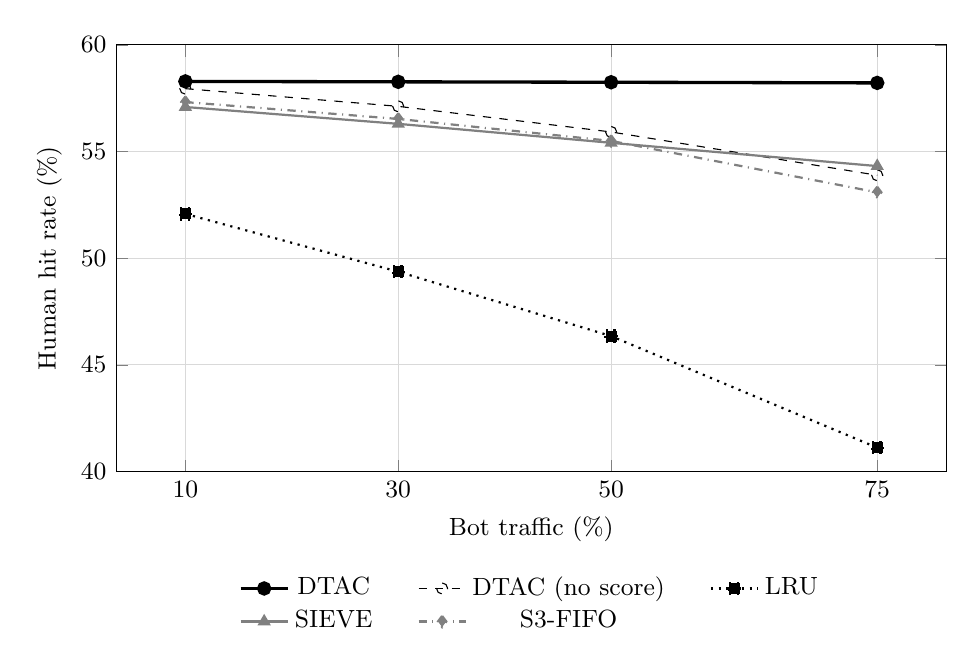
\begin{tikzpicture}
        \begin{axis}[resultaxis, xlabel={Bot traffic (\%)}, ylabel={Human hit rate (\%)}, ymin=40, ymax=60]
            \addplot[algdtac] coordinates {(10,58.29) (30,58.27) (50,58.25) (75,58.22)};
            \addplot[algnoscore] coordinates {(10,57.95) (30,57.12) (50,55.92) (75,53.89)};
            \addplot[alglru] coordinates {(10,52.08) (30,49.37) (50,46.35) (75,41.12)};
            \addplot[algsieve] coordinates {(10,57.09) (30,56.30) (50,55.41) (75,54.32)};
            \addplot[algsfifo] coordinates {(10,57.32) (30,56.53) (50,55.50) (75,53.09)};
            \legend{DTAC, DTAC (no score), LRU, SIEVE, S3-FIFO}
        \end{axis}
    \end{tikzpicture}
    \caption{Human hit rate against bot traffic share, naive workload, capacity 10{,}000}
    \label{fig:hhr-naive}
\end{figure}

DTAC's human hit rate was essentially unaffected by the volume of naive bot traffic: it fell by only 0.07 percentage points, from 58.29\% at 10\% bots to 58.22\% at 75\%, which is within the confidence intervals. Every other algorithm degraded as the bot share grew. LRU lost 10.96 points (from 52.08\% to 41.12\%), S3-FIFO 4.23 points, the DTAC ablation 4.06 points and SIEVE 2.77 points. DTAC had the highest human hit rate at every ratio.

Table~\ref{tab:paired-naive} gives the paired per-seed differences between DTAC and each alternative. Every difference was positive and every confidence interval excluded zero.

\begin{table}[htbp]
    \centering
    \caption{Paired difference in human hit rate, DTAC $-$ X (percentage points), naive workload, capacity 10{,}000. Bold: 95\% CI excludes zero}
    \label{tab:paired-naive}
    \small
    \begin{tabular}{lcccc}
        \toprule
        Bot ratio & vs DTAC (no score) & vs LRU & vs SIEVE & vs S3-FIFO \\
        \midrule
        10\% & \textbf{+0.33} $\pm$ 0.04 & \textbf{+6.21} $\pm$ 0.10 & \textbf{+1.19} $\pm$ 0.11 & \textbf{+0.97} $\pm$ 0.14 \\
        30\% & \textbf{+1.15} $\pm$ 0.13 & \textbf{+8.90} $\pm$ 0.15 & \textbf{+1.97} $\pm$ 0.06 & \textbf{+1.74} $\pm$ 0.09 \\
        50\% & \textbf{+2.33} $\pm$ 0.08 & \textbf{+11.90} $\pm$ 0.12 & \textbf{+2.84} $\pm$ 0.15 & \textbf{+2.75} $\pm$ 0.05 \\
        75\% & \textbf{+4.33} $\pm$ 0.21 & \textbf{+17.10} $\pm$ 0.22 & \textbf{+3.90} $\pm$ 0.15 & \textbf{+5.13} $\pm$ 0.14 \\
        \bottomrule
    \end{tabular}
\end{table}

Two observations follow from these tables. First, the advantage over every alternative grew with the bot share: over LRU from 6.21 to 17.10 points, over SIEVE from 1.19 to 3.90 and over S3-FIFO from 0.97 to 5.13. Second, the comparison with the ablation isolates the contribution of the AI-score, since the two configurations share the same engine and differ only in whether bots can be told apart. That contribution also grew with the bot share, from 0.33 points at 10\% to 4.33 points at 75\%. The ablation on its own was already competitive with the scan-resistant baselines: it was ahead of both SIEVE and S3-FIFO at 10--50\% bots and between them at 75\% (53.89\% against 54.32\% and 53.09\%). Most of DTAC's margin over SIEVE and S3-FIFO is therefore attributable to the AI-score rather than to the ghost cache and the decayed-score tournament alone.

\section{Secondary Metrics under Naive Scrapers}
Table~\ref{tab:secondary-naive} reports the overall hit rate (over human and bot requests together), the human byte hit rate and, for reference only, the bot hit rate.

\begin{table}[htbp]
    \centering
    \caption{Secondary metrics (\%), naive workload, capacity 10{,}000}
    \label{tab:secondary-naive}
    \small
    \begin{tabular}{llccccc}
        \toprule
        Metric & Bot ratio & DTAC & DTAC (no score) & LRU & SIEVE & S3-FIFO \\
        \midrule
        Overall hit rate & 10\% & 53.31 & 53.03 & 47.84 & 52.31 & 52.52 \\
         & 30\% & 43.49 & 42.76 & 37.48 & 42.34 & 42.48 \\
         & 50\% & 33.71 & 32.74 & 28.10 & 32.62 & 32.65 \\
         & 75\% & 21.47 & 20.81 & 17.73 & 21.00 & 20.71 \\
        \midrule
        Human byte hit rate & 10\% & 53.11 & 52.67 & 46.04 & 51.73 & 51.95 \\
         & 30\% & 53.08 & 51.68 & 42.96 & 50.78 & 50.99 \\
         & 50\% & 53.05 & 50.51 & 39.43 & 49.77 & 49.88 \\
         & 75\% & 53.07 & 48.12 & 33.54 & 48.56 & 47.20 \\
        \midrule
        Bot hit rate & 10\% & 9.12 & 9.27 & 10.12 & 9.86 & 9.83 \\
        (reference only) & 30\% & 9.20 & 9.47 & 9.93 & 9.95 & 9.92 \\
         & 50\% & 9.29 & 9.69 & 9.95 & 9.95 & 9.92 \\
         & 75\% & 9.28 & 9.83 & 9.97 & 9.95 & 9.97 \\
        \bottomrule
    \end{tabular}
\end{table}

The overall hit rate necessarily falls for every algorithm as the bot share grows, because bot requests are mostly for objects that are not cached. DTAC nevertheless had the highest overall hit rate at every ratio; the paired differences against every alternative were positive with confidence intervals excluding zero (for example $+0.47 \pm 0.10$ points over SIEVE and $+3.74 \pm 0.09$ over LRU at 75\% bots). This is despite DTAC serving bots slightly less often (a bot hit rate of about 9.2\% against about 10\% for the baselines), because humans account for most cache hits.

The human byte hit rate followed the human hit rate closely. DTAC's human byte hit rate stayed between 53.05\% and 53.11\% at every ratio, while LRU's fell from 46.04\% to 33.54\%. The confidence intervals for this metric were between 0.17 and 0.69 points. As noted in Section 3.7.1, none of the algorithms is size-aware, so this metric reflects how hits on popular objects correlate with their size rather than any deliberate byte-level optimization.

\section{Results under Stealthy Scrapers}
Table~\ref{tab:hhr-stealthy} and Figure~\ref{fig:hhr-stealthy} show the human hit rate for the stealthy workload, against which the router performed no better than chance (Section 4.3).

\begin{table}[htbp]
    \centering
    \caption{Human cache hit rate (\%), stealthy workload, capacity 10{,}000}
    \label{tab:hhr-stealthy}
    \small
    \begin{tabular}{lccccc}
        \toprule
        Bot ratio & DTAC & DTAC (no score) & LRU & SIEVE & S3-FIFO \\
        \midrule
        10\% & 57.96 $\pm$ 0.15 & 58.04 $\pm$ 0.16 & 52.34 $\pm$ 0.21 & 57.21 $\pm$ 0.14 & 57.40 $\pm$ 0.21 \\
        30\% & 57.34 $\pm$ 0.09 & 57.31 $\pm$ 0.16 & 50.03 $\pm$ 0.22 & 56.52 $\pm$ 0.06 & 56.70 $\pm$ 0.14 \\
        50\% & 56.34 $\pm$ 0.10 & 56.32 $\pm$ 0.13 & 47.27 $\pm$ 0.23 & 55.71 $\pm$ 0.10 & 55.82 $\pm$ 0.17 \\
        75\% & 54.40 $\pm$ 0.11 & 54.36 $\pm$ 0.09 & 42.29 $\pm$ 0.27 & 54.53 $\pm$ 0.22 & 53.81 $\pm$ 0.12 \\
        \bottomrule
    \end{tabular}
\end{table}

\begin{figure}[htbp]
    \centering
    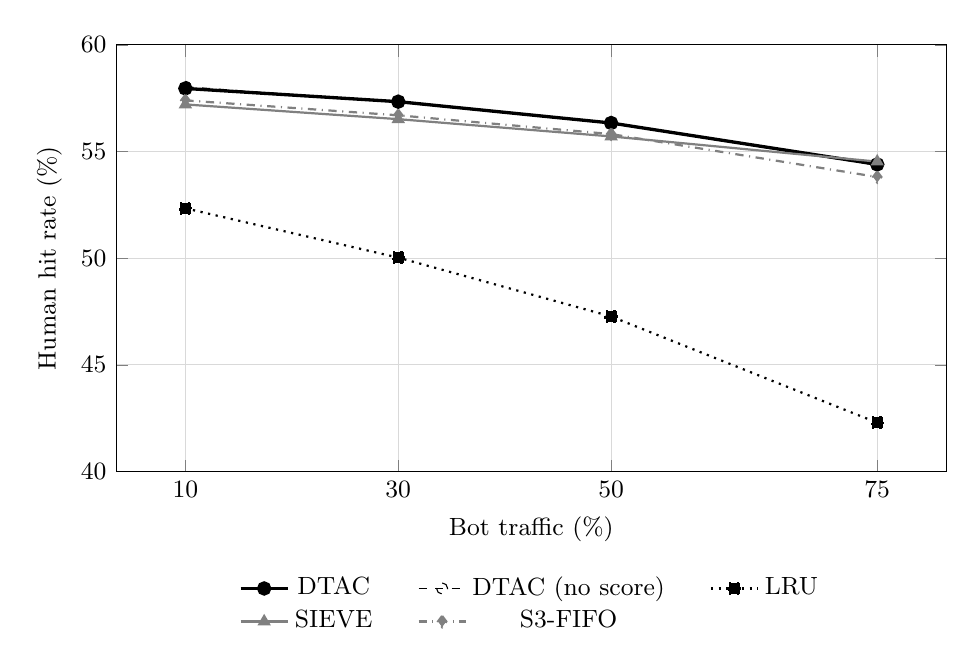
\begin{tikzpicture}
        \begin{axis}[resultaxis, xlabel={Bot traffic (\%)}, ylabel={Human hit rate (\%)}, ymin=40, ymax=60]
            \addplot[algdtac] coordinates {(10,57.96) (30,57.34) (50,56.34) (75,54.40)};
            \addplot[algnoscore] coordinates {(10,58.04) (30,57.31) (50,56.32) (75,54.36)};
            \addplot[alglru] coordinates {(10,52.34) (30,50.03) (50,47.27) (75,42.29)};
            \addplot[algsieve] coordinates {(10,57.21) (30,56.52) (50,55.71) (75,54.53)};
            \addplot[algsfifo] coordinates {(10,57.40) (30,56.70) (50,55.82) (75,53.81)};
            \legend{DTAC, DTAC (no score), LRU, SIEVE, S3-FIFO}
        \end{axis}
    \end{tikzpicture}
    \caption{Human hit rate against bot traffic share, stealthy workload, capacity 10{,}000}
    \label{fig:hhr-stealthy}
\end{figure}

\begin{table}[htbp]
    \centering
    \caption{Paired difference in human hit rate, DTAC $-$ X (percentage points), stealthy workload, capacity 10{,}000. Bold: 95\% CI excludes zero}
    \label{tab:paired-stealthy}
    \small
    \begin{tabular}{lcccc}
        \toprule
        Bot ratio & vs DTAC (no score) & vs LRU & vs SIEVE & vs S3-FIFO \\
        \midrule
        10\% & \textbf{$-$0.08} $\pm$ 0.05 & \textbf{+5.62} $\pm$ 0.11 & \textbf{+0.75} $\pm$ 0.14 & \textbf{+0.56} $\pm$ 0.08 \\
        30\% & +0.03 $\pm$ 0.09 & \textbf{+7.31} $\pm$ 0.14 & \textbf{+0.82} $\pm$ 0.05 & \textbf{+0.64} $\pm$ 0.09 \\
        50\% & +0.02 $\pm$ 0.05 & \textbf{+9.07} $\pm$ 0.16 & \textbf{+0.64} $\pm$ 0.14 & \textbf{+0.52} $\pm$ 0.15 \\
        75\% & +0.04 $\pm$ 0.11 & \textbf{+12.11} $\pm$ 0.23 & $-$0.13 $\pm$ 0.18 & \textbf{+0.59} $\pm$ 0.18 \\
        \bottomrule
    \end{tabular}
\end{table}

With the router unable to identify the bots, DTAC and its ablation behaved identically within measurement error (Table~\ref{tab:paired-stealthy}): the differences at 30--75\% were statistically indistinguishable from zero, and at 10\% the ablation was very slightly ahead ($-0.08 \pm 0.05$ points). DTAC's human hit rate was no longer stable, falling by 3.56 points from 57.96\% to 54.40\% as the bot share rose, a decline comparable to SIEVE's (2.68 points) and S3-FIFO's (3.59 points).

DTAC still outperformed LRU at every ratio (by 5.62 to 12.11 points) and S3-FIFO by about 0.5--0.6 points, and it outperformed SIEVE at 10--50\% bots. At 75\% it tied with SIEVE ($-0.13 \pm 0.18$). Since the AI-score contributed nothing on this workload, these remaining advantages come from the engine's ghost-cache admission and long-memory tournament alone. For the overall hit rate, DTAC was slightly behind SIEVE at 75\% bots ($-0.15 \pm 0.09$ points).

The bot hit rate on this workload was about 28\% for every algorithm (27.47--28.08\%), much higher than for naive bots, because each stealthy IP fetches the favicon, which is always cached, in addition to its uniformly scanned pages. The human byte hit rate again tracked the human hit rate (48.86\% for DTAC at 75\% bots, against 48.83\% for SIEVE and 34.86\% for LRU).

\section{Effect of Cache Capacity}
Table~\ref{tab:capacity} and Figure~\ref{fig:capacity} show the human hit rate on the naive workload at capacities from 1\% to 20\% of the catalog, at 30\% and 75\% bot traffic. The shard count was chosen automatically (8, 64, 128 and 256 shards respectively), and the constants calibrated at 10{,}000 entries were used at every capacity.

\begin{table}[htbp]
    \centering
    \caption{Human cache hit rate (\%) against cache capacity, naive workload}
    \label{tab:capacity}
    \small
    \begin{tabular}{llccccc}
        \toprule
        Bot ratio & Capacity & DTAC & DTAC (no score) & LRU & SIEVE & S3-FIFO \\
        \midrule
        30\% & 1{,}000 & 39.41 & 39.17 & 27.61 & 38.27 & \textbf{39.48} \\
         & 5{,}000 & \textbf{51.95} & 50.91 & 40.92 & 49.89 & 50.74 \\
         & 10{,}000 & \textbf{58.27} & 57.12 & 49.37 & 56.30 & 56.53 \\
         & 20{,}000 & 61.50 & 62.56 & 60.50 & \textbf{64.48} & 63.74 \\
        \midrule
        75\% & 1{,}000 & \textbf{39.38} & 37.62 & 22.07 & 37.71 & 37.75 \\
         & 5{,}000 & \textbf{51.85} & 48.43 & 33.26 & 48.36 & 47.61 \\
         & 10{,}000 & \textbf{58.22} & 53.89 & 41.12 & 54.32 & 53.09 \\
         & 20{,}000 & 61.49 & 61.01 & 52.21 & \textbf{62.10} & 60.42 \\
        \bottomrule
    \end{tabular}
\end{table}

\begin{figure}[htbp]
    \centering
    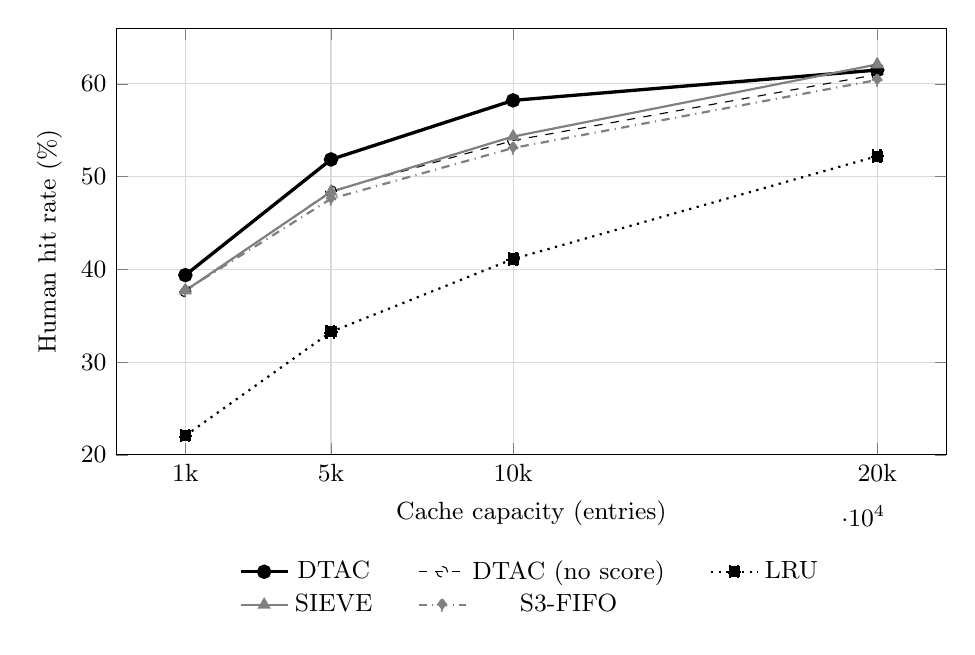
\begin{tikzpicture}
        \begin{axis}[resultaxis, xlabel={Cache capacity (entries)}, ylabel={Human hit rate (\%)}, xtick={1000,5000,10000,20000}, xticklabels={1k,5k,10k,20k}, ymin=20, ymax=66]
            \addplot[algdtac] coordinates {(1000,39.38) (5000,51.85) (10000,58.22) (20000,61.49)};
            \addplot[algnoscore] coordinates {(1000,37.62) (5000,48.43) (10000,53.89) (20000,61.01)};
            \addplot[alglru] coordinates {(1000,22.07) (5000,33.26) (10000,41.12) (20000,52.21)};
            \addplot[algsieve] coordinates {(1000,37.71) (5000,48.36) (10000,54.32) (20000,62.10)};
            \addplot[algsfifo] coordinates {(1000,37.75) (5000,47.61) (10000,53.09) (20000,60.42)};
            \legend{DTAC, DTAC (no score), LRU, SIEVE, S3-FIFO}
        \end{axis}
    \end{tikzpicture}
    \caption{Human hit rate against cache capacity, naive workload, 75\% bot traffic}
    \label{fig:capacity}
\end{figure}

\begin{table}[htbp]
    \centering
    \caption{Paired difference in human hit rate, DTAC $-$ X (percentage points), against cache capacity, naive workload. Every 95\% CI excludes zero (half-widths 0.05--0.36)}
    \label{tab:paired-capacity}
    \small
    \begin{tabular}{llcccc}
        \toprule
        Bot ratio & Capacity & vs DTAC (no score) & vs LRU & vs SIEVE & vs S3-FIFO \\
        \midrule
        30\% & 1{,}000 & +0.24 & +11.80 & +1.14 & $-$0.07 \\
         & 5{,}000 & +1.04 & +11.03 & +2.06 & +1.21 \\
         & 10{,}000 & +1.15 & +8.90 & +1.97 & +1.74 \\
         & 20{,}000 & $-$1.07 & +1.00 & $-$2.99 & $-$2.24 \\
        \midrule
        75\% & 1{,}000 & +1.76 & +17.32 & +1.67 & +1.64 \\
         & 5{,}000 & +3.42 & +18.59 & +3.49 & +4.24 \\
         & 10{,}000 & +4.33 & +17.10 & +3.90 & +5.13 \\
         & 20{,}000 & +0.49 & +9.28 & $-$0.61 & +1.08 \\
        \bottomrule
    \end{tabular}
\end{table}

From 1{,}000 to 10{,}000 entries, DTAC outperformed every baseline on the naive workload, with the single exception of S3-FIFO at 1{,}000 entries and 30\% bots, where S3-FIFO was ahead by a statistically significant but practically negligible 0.07 points. At 75\% bots its advantage over SIEVE and S3-FIFO was largest at 5{,}000 and 10{,}000 entries (3.5--5.1 points).

At 20{,}000 entries (20\% of the catalog) the picture changed. DTAC still beat LRU (by 1.00 and 9.28 points), but it lost to SIEVE at both bot ratios ($-2.99$ points at 30\% and $-0.61$ at 75\%) and, at 30\% bots, to S3-FIFO ($-2.24$) and even to its own ablation ($-1.07$). Its human hit rate also grew less with capacity than the baselines' did: from 10{,}000 to 20{,}000 entries DTAC gained about 3.3 points, against about 8 points for SIEVE at both ratios. Its overall hit rate at 20{,}000 entries was lower than that of every other algorithm, including LRU (by 1.55 points at 30\% bots and 3.22 points at 75\%). The calibration check reported in Section 3.4.3 had already shown that, at this capacity, a lower promotion threshold would have improved DTAC's human hit rate by about 2.3 points. No algorithm showed a sudden drop at the smallest capacity, indicating that the small shards used there (8 shards of 125 entries) did not distort the results.

\section{Cache Pollution}
Table~\ref{tab:cpi} and Figure~\ref{fig:cpi} report the Cache Pollution Index, the share of resident main-cache entries that no human had requested since their admission.

\begin{table}[htbp]
    \centering
    \caption{Cache Pollution Index (\%), capacity 10{,}000}
    \label{tab:cpi}
    \small
    \begin{tabular}{llccccc}
        \toprule
        Workload & Bot ratio & DTAC & DTAC (no score) & LRU & SIEVE & S3-FIFO \\
        \midrule
        Naive & 10\% & 0.0 & 6.0 & 14.0 & 7.0 & 8.6 \\
         & 30\% & 0.0 & 17.9 & 37.4 & 18.3 & 23.0 \\
         & 50\% & 0.0 & 30.5 & 57.2 & 27.7 & 36.2 \\
         & 75\% & 0.0 & 47.6 & 78.9 & 37.4 & 55.3 \\
        \midrule
        Stealthy & 10\% & 4.9 & 4.9 & 11.4 & 5.7 & 7.0 \\
         & 30\% & 15.1 & 15.2 & 32.2 & 15.8 & 20.0 \\
         & 50\% & 26.6 & 26.6 & 51.6 & 25.1 & 32.3 \\
         & 75\% & 43.9 & 44.1 & 74.9 & 35.7 & 50.9 \\
        \bottomrule
    \end{tabular}
\end{table}

\begin{figure}[htbp]
    \centering
    \begin{minipage}{0.49\textwidth}
        \centering
        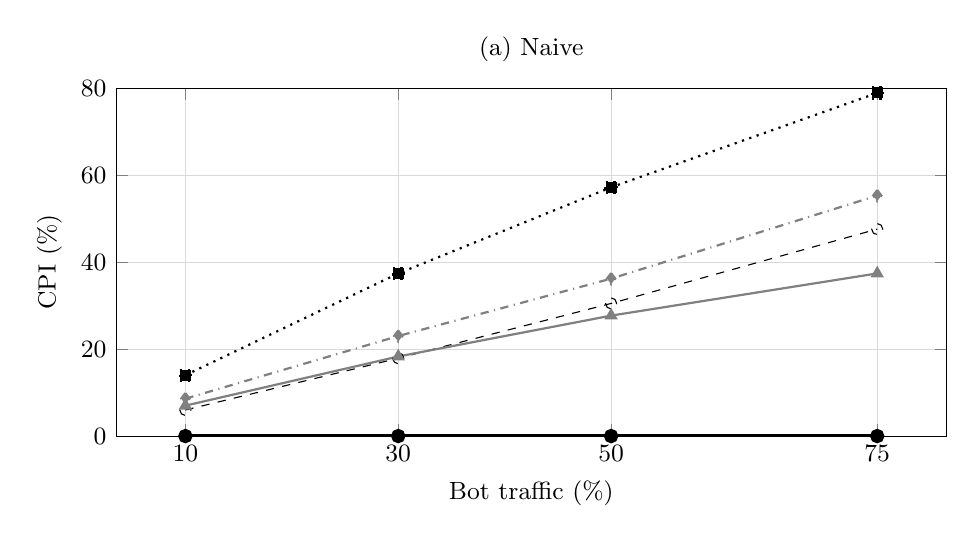
\begin{tikzpicture}
            \begin{axis}[resultaxis, height=6cm, title={(a) Naive}, xlabel={Bot traffic (\%)}, ylabel={CPI (\%)}, ymin=0, ymax=80, legend to name=cpilegend]
                \addplot[algdtac] coordinates {(10,0.0) (30,0.0) (50,0.0) (75,0.0)};
                \addplot[algnoscore] coordinates {(10,6.0) (30,17.9) (50,30.5) (75,47.6)};
                \addplot[alglru] coordinates {(10,14.0) (30,37.4) (50,57.2) (75,78.9)};
                \addplot[algsieve] coordinates {(10,7.0) (30,18.3) (50,27.7) (75,37.4)};
                \addplot[algsfifo] coordinates {(10,8.6) (30,23.0) (50,36.2) (75,55.3)};
                \legend{DTAC, DTAC (no score), LRU, SIEVE, S3-FIFO}
            \end{axis}
        \end{tikzpicture}
    \end{minipage}\hfill
    \begin{minipage}{0.49\textwidth}
        \centering
        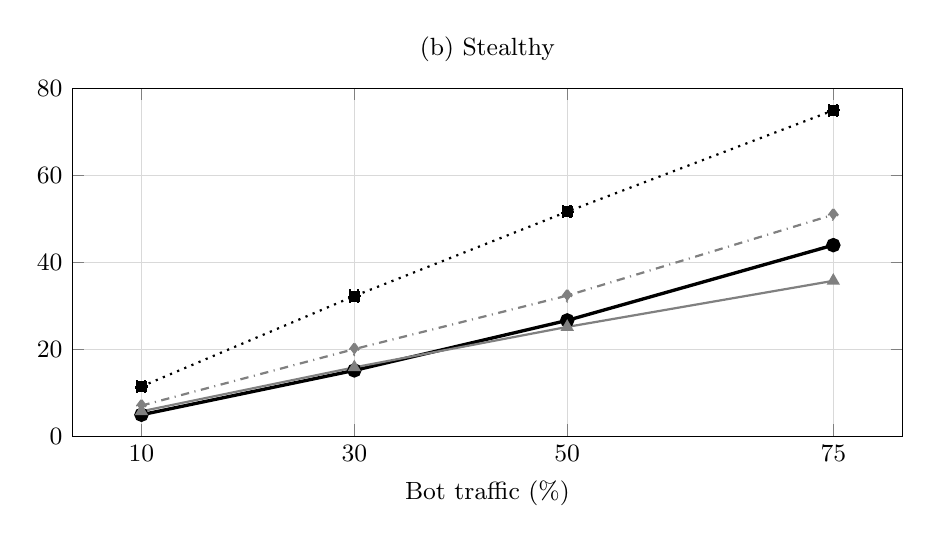
\begin{tikzpicture}
            \begin{axis}[resultaxis, height=6cm, title={(b) Stealthy}, xlabel={Bot traffic (\%)}, ymin=0, ymax=80]
                \addplot[algdtac] coordinates {(10,4.9) (30,15.1) (50,26.6) (75,43.9)};
                \addplot[algnoscore] coordinates {(10,4.9) (30,15.2) (50,26.6) (75,44.1)};
                \addplot[alglru] coordinates {(10,11.4) (30,32.2) (50,51.6) (75,74.9)};
                \addplot[algsieve] coordinates {(10,5.7) (30,15.8) (50,25.1) (75,35.7)};
                \addplot[algsfifo] coordinates {(10,7.0) (30,20.0) (50,32.3) (75,50.9)};
            \end{axis}
        \end{tikzpicture}
    \end{minipage}
    \ref{cpilegend}
    \caption{Cache Pollution Index against bot traffic share, capacity 10{,}000}
    \label{fig:cpi}
\end{figure}

On the naive workload DTAC's CPI was exactly zero at every bot ratio and in every seed: no item requested only by bots was ever admitted to the main cache, because detected bot requests contribute almost nothing to a resource's score and so cannot promote it. The share of resident entries whose admission had been triggered by a bot request was likewise zero. For every other algorithm the CPI grew roughly in proportion to the bot share. At 75\% bots, 78.9\% of LRU's capacity held content that no human had requested since admission, against 55.3\% for S3-FIFO, 47.6\% for the ablation and 37.4\% for SIEVE.

On the stealthy workload DTAC's CPI matched its ablation's at every ratio (4.9--44.1\%), was well below LRU's and S3-FIFO's, and was close to SIEVE's at 10--50\% bots. At 75\% bots SIEVE retained noticeably less bot-only content (35.7\%) than DTAC (43.9\%).

\section{Latency and Memory Overhead}
Table~\ref{tab:overhead} summarizes the computational and memory overhead at a capacity of 10{,}000 entries. $T_{proxy}$ is the router's scoring time per request and applies only to DTAC. The total access time includes the router (for DTAC), the cache engine and the replayer's own metric recording; for DTAC it also includes the system's built-in telemetry, which runs after both phase timers stop. The memory figure is the growth of the process's resident set size over the replay, which reflects cache metadata (and the replayer's own bookkeeping, identical for every algorithm) but not payload bytes.

\begin{table}[htbp]
    \centering
    \caption{Latency (99th percentile, $\mu$s) and memory overhead (RSS growth over the replay), capacity 10{,}000}
    \label{tab:overhead}
    \small
    \setlength{\tabcolsep}{4pt}
    \begin{tabular}{llccccc}
        \toprule
        Metric & Workload, ratio & DTAC & DTAC (no score) & LRU & SIEVE & S3-FIFO \\
        \midrule
        $T_{proxy}$ p99 & Naive, 10--75\% & 22.8--35.0 & -- & -- & -- & -- \\
         & Stealthy, 10--75\% & 35.3--39.2 & -- & -- & -- & -- \\
        \midrule
        Total p99 & Naive, 30\% & 160 & 112 & 87 & 82 & 124 \\
         & Naive, 75\% & 92 & 93 & 79 & 80 & 88 \\
         & Stealthy, 30\% & 141 & 105 & 100 & 85 & 89 \\
         & Stealthy, 75\% & 148 & 93 & 120 & 107 & 92 \\
        \midrule
        RSS (MiB) & Naive, 10\% & 17.1 & 12.9 & 4.8 & 4.9 & 8.6 \\
         & Naive, 75\% & 32.5 & 20.4 & 4.8 & 4.9 & 9.1 \\
         & Stealthy, 75\% & 28.9 & 19.7 & 4.6 & 5.0 & 9.1 \\
        \midrule
        Ghost entries & Naive, 10\% & 35{,}340 & 32{,}634 & -- & -- & 8{,}916 \\
         & Naive, 75\% & 79{,}530 & 44{,}883 & -- & -- & 8{,}928 \\
         & Stealthy, 75\% & 44{,}926 & 44{,}861 & -- & -- & 8{,}932 \\
        \bottomrule
    \end{tabular}
\end{table}

The router's 99th-percentile scoring time was between 22.8 and 39.2 microseconds across all cells, roughly fifty times below the 2-millisecond budget set in Section 3.7.4. The 99th-percentile total access time was below 0.2 milliseconds for every algorithm. These tail latencies were noisy across seeds: the 95\% confidence half-widths ranged from about 13 to 87 microseconds, so most differences between algorithms in Table~\ref{tab:overhead} are not statistically meaningful. DTAC's total tail latency was nonetheless typically higher than the baselines', by up to about 100 microseconds in the noisiest cells, consistent with the additional router work and telemetry on its path.

DTAC used more memory than the baselines. Its RSS growth was 17.1 MiB at 10\% naive bots and 32.5 MiB at 75\%, against about 5 MiB for LRU and SIEVE and about 9 MiB for S3-FIFO. The difference is almost entirely the ghost cache and the router's per-IP state. DTAC's ghost cache grew with the naive bot share, from 35{,}340 entries at 10\% to 79{,}530 at 75\%, close to its bound of eight times the main-cache capacity (79{,}872 entries), because every detected bot miss leaves a near-zero-score ghost entry; the ablation's ghost held about 45{,}000 entries. All algorithms held the same 9{,}984 main-cache entries and about 256 MiB of logical payload, so the comparison is at equal main-cache capacity.

\section{Networked Validation}
To confirm that the in-process replay reflects the behavior of the deployed system, seed 1's naive log at 30\% bots was also replayed over HTTP on \texttt{localhost}, through the standalone DTAC reverse proxy to the stub origin server, at a capacity of 10{,}000 entries. The networked run gave a human hit rate of 58.29\% against 58.32\% in-process for the same seed, both within the five-seed interval of $58.27 \pm 0.12\%$. The overall hit rate was 43.44\% against 43.46\%, and the router's class-mean gap was 0.975 in both cases. Over HTTP the whole round trip took 2.8 milliseconds at the median and 9.7 milliseconds at the 99th percentile, at about 33{,}000 requests per second, against a 99th percentile of about 0.2 milliseconds in-process. This additional time is the cost of the HTTP stack and the network loopback, not of the cache or the router.

\section{Summary of Results}
The main findings of the experiments are as follows:
\begin{enumerate}
    \item Against naive scrapers, the router separated bots from humans perfectly (ROC-AUC 1.000, class-mean gap 0.976) with no false positives at a threshold of 0.5, although returning visitors were penalized slightly.
    \item With this separation, DTAC's human hit rate stayed at 58.2--58.3\% at a capacity of 10{,}000 entries regardless of the bot share, while every alternative degraded. At 75\% bots DTAC outperformed LRU by 17.10 points, SIEVE by 3.90, S3-FIFO by 5.13 and its own no-score ablation by 4.33, with every difference statistically significant.
    \item The ablation showed that the AI-score is responsible for most of DTAC's advantage over the scan-resistant baselines, and that this contribution grows with the bot share.
    \item DTAC admitted no bot-only content on the naive workload (CPI 0.0\%), against 37--79\% for the baselines at 75\% bots.
    \item Against stealthy scrapers the router was no better than chance (ROC-AUC 0.485), DTAC tied its ablation, and its human hit rate declined like SIEVE's. It still outperformed LRU and S3-FIFO and tied SIEVE at 75\% bots.
    \item DTAC's advantage depended on cache capacity: it led at 1--10\% of the catalog but lost to SIEVE (and, at 30\% bots, to S3-FIFO and its ablation) at 20\%, where its constants were known to be suboptimal.
    \item The overhead was modest: router scoring took 23--39 $\mu$s at the 99th percentile, total tail latency stayed below 0.2 ms, and DTAC's metadata used up to about 28 MiB more memory than LRU, mainly for its ghost cache.
    \item A networked replay through the real proxy reproduced the in-process hit rates to within 0.03 points.
\end{enumerate}

\chapter{Discussion, Conclusion and Recommendations}
\label{chap:discussion}

\section{Introduction}
This chapter interprets the results presented in Chapter~\ref{chap:results} in the light of the literature reviewed in Chapter~\ref{chap:literature_review} and the objectives set out in Chapter~\ref{chap:introduction}. Section 5.2 discusses the main findings and what they reveal about the design of the system. Section 5.3 evaluates the extent to which each research objective was achieved, and Section 5.4 states the contributions of the study. Section 5.5 sets out its limitations, Section 5.6 offers recommendations for practitioners, Section 5.7 proposes directions for future work, and Section 5.8 concludes the thesis.

\section{Discussion of Findings}

\subsection{The AI-Score Protects Human Hit Rate When Bots Are Detectable}
The central hypothesis of this study was that feeding a real-time bot-probability score into a cache's admission and eviction logic would preserve the cache's usefulness to human users during heavy scraper activity. The naive-workload results support this hypothesis strongly. DTAC's human hit rate was the same, within measurement error, at 10\% and at 75\% bot traffic (58.29\% and 58.22\%), while LRU lost 11 points over the same range. In effect, detected scrapers were made invisible to the cache: their requests contributed almost nothing to any resource's score, so they never caused an admission (a Cache Pollution Index of exactly zero) and could not displace human content.

The ablation is what allows this effect to be attributed to the AI-score itself rather than to other features of the engine. The no-score variant shares DTAC's ghost cache, decay and eviction tournament and differs only in that it cannot tell bots from humans. The gap between the two grew steadily with the bot share, from 0.33 points at 10\% to 4.33 points at 75\%, while on the stealthy workload, where the router could not distinguish the classes, the gap vanished (between $-0.08$ and $+0.04$ points). These two results together form a natural control: the score helps exactly when, and roughly in proportion to how much, it carries information about which requests are bots.

\subsection{Comparison with Scan-Resistant Algorithms}
\citeA{zhang_rethinking_2026} reported that, under AI scan traffic, ``smarter eviction algorithms can serve as lightweight traffic filters'', with SIEVE, S3-FIFO and ARC degrading far more gracefully than LRU, LFU and FIFO. The present results reproduce that ordering: SIEVE and S3-FIFO outperformed LRU by 12--13 points of human hit rate at 75\% naive bots, and their human hit rate fell by only 2.8 and 4.2 points between 10\% and 75\% bots against LRU's 11. The absolute hit rates are lower than the 70--80\% reported by \citeA{zhang_rethinking_2026} for pure human traffic, because the workloads differ (here the catalog has 100{,}000 objects with a Zipf exponent of 0.8 and the cache holds 10\% of it), but the qualitative behavior is the same. The finding of \citeA{zhang_rethinking_2026} that overall hit ratios fall below 30\% for all policies at a 75\% scan ratio is also visible: at 75\% naive bots no algorithm, DTAC included, exceeded an overall hit rate of 22\%. This is not a failure of the caches; when three quarters of requests are for uniformly scanned objects that will rarely be requested again, most of those requests cannot be hits under any policy. This observation supports the choice of the human hit rate, rather than the overall hit rate, as the primary metric.

Chapter 2 argued that structural scan resistance is ``naive to the origin of the request'' and infers bot-like behavior only from access patterns after the cache is already under pressure. The results quantify the value of adding explicit origin information. On naive bots, DTAC improved on SIEVE by 1.2--3.9 points and on S3-FIFO by 1.0--5.1 points at 10{,}000 entries, and it eliminated cache pollution where SIEVE still allowed 37\% of the cache to be occupied by bot-only content at 75\% bots. It is worth noting, however, that the ablation alone was already roughly on par with SIEVE and S3-FIFO. The engine's two-stage admission, which follows the same intuition as S3-FIFO's small queue and ghost queue \cite{yang_fifo_2023} and TinyLFU's frequency-based admission filter \cite{einziger_tinylfu_2017}, provides most of the structural scan resistance on its own; the AI-score then adds a further, bot-specific layer on top of it.

\subsection{The Engine Behaves Like a Human-Weighted LFU}
Calibration chose a score half-life of four hours, longer than the benchmark logs themselves. Within a replay, therefore, scores barely decay and the engine behaves as a Least Frequently Used policy in which each request is weighted by how human it appears, with recency used only to break ties. Chapter 2 noted that LFU is well suited to static, heavily skewed popularity but suffers from ``frequency pollution'' when popularity changes. The synthetic workloads used here have stationary Zipf popularity, which is precisely the setting that favors LFU. The decay mechanism is what is meant to protect DTAC from frequency pollution on real, drifting workloads, but this study did not evaluate a drifting workload, and the calibrated half-life is likely too long for one. This is an important qualification of the results (Section 5.5).

\subsection{The Limits of Passive Heuristics}
The stealthy workload was designed to show where the heuristics stop working, and the result was unambiguous: with browser headers, residential addresses, a handful of requests per IP and a single favicon fetch, the bots scored marginally \emph{lower} than humans (ROC-AUC 0.485). Each of the four signals is defeated by a simple, cheap change in scraper behavior. The header check tests only for the presence of \texttt{Accept-Language}; the datacenter test is defeated by residential proxies; the velocity and ``Shy Guys'' heuristics both operate per IP and are defeated by rotating addresses, and ``Shy Guys'' additionally needs only one asset fetch per IP. This is consistent with the literature reviewed in Chapter 2: \citeA{ousat_broken_2026} document how modern bots evade even active challenges, and \citeA{hoetzlein_protecting_2025} motivate subnet-level aggregation precisely because per-IP rate limiting is evaded by distributing requests across many addresses. \citeA{van_boxem_shy_2026} present the structural favicon heuristic as a lightweight signal in combination with others, not as a robust one on its own.

The important practical point is that DTAC degraded gracefully when its detector failed. Because an undetected bot is simply treated as a human, DTAC on the stealthy workload behaved exactly like its ablation, which still outperformed LRU and S3-FIFO and tied SIEVE at 75\% bots. A wrong or uninformative score does not make the cache worse than a well-designed score-blind cache; it only removes the additional benefit. The converse risk, penalizing humans, was also small in these experiments: although returning visitors were penalized slightly (mean bot probability 0.030 against 0.021 for new visitors), a human contribution of 0.97 instead of 0.98 per request is immaterial to the cache, and no human crossed a bot probability of 0.5.

\subsection{Sensitivity to Cache Capacity}
DTAC's advantage was not uniform across cache sizes. At 20{,}000 entries it lost to SIEVE at both bot ratios and, at 30\% bots, to S3-FIFO and to its own ablation. Two factors visible in the data explain this. First, the constants were calibrated at 10{,}000 entries, and the calibration check showed that at 20{,}000 a promotion threshold of 0.5 (admitting on the first human request) would have been about 2.3 points better than the calibrated 1.5. With a large cache relative to the catalog, the requirement that an object be requested twice by humans before admission costs more hits than it saves. Second, with 20\% of the catalog cached, the scan-resistant baselines lose comparatively little to bots in the first place, so there is less pollution for the AI-score to prevent. That DTAC's overall hit rate at this capacity fell even below LRU's reflects the same strict admission: objects requested once by a human, or requested mostly by bots, are never admitted, so DTAC forgoes hits that a permissive policy collects. These results show that DTAC's parameters, in particular its promotion threshold, should be tuned to the cache's size relative to its working set, as the literature on adaptive cache management suggests \cite{vysotska_towards_2025}.

\subsection{Cost of the Approach}
The overhead of the approach was modest. The router took 23--39 microseconds at the 99th percentile, far below the 2-millisecond budget set in Chapter~\ref{chap:methodology} and far below the 2.8-millisecond median round trip of even a loopback HTTP request. This confirms the argument of Chapter 2 that composite trust scoring built only from cheap, passive signals can be placed on the critical path of a cache \cite{chandra_composite_2026}. The main cost was memory: DTAC's metadata grew by up to 32.5 MiB against about 5 MiB for LRU, mostly because the ghost cache, bounded at eight times the main capacity, fills up with near-zero-score entries left by bot misses. The additional 28 MiB over LRU amounts to about 11\% of the roughly 256 MiB of payload held in the main cache; it is the price of the long ghost memory that the calibration found beneficial.

\section{Evaluation against the Research Objectives}
Table~\ref{tab:objectives} summarizes the extent to which each specific objective stated in Section 1.3.2 was achieved.

\begin{table}[htbp]
    \centering
    \caption{Status of the research objectives}
    \label{tab:objectives}
    \small
    \begin{tabular}{p{0.3\textwidth}p{0.17\textwidth}p{0.43\textwidth}}
        \toprule
        Objective & Status & Evidence \\
        \midrule
        1. Build a lightweight heuristic detector using passive analysis of header anomalies and structural requests & Achieved against naive bots; not against stealthy bots & Four passive heuristics (velocity, \texttt{Accept-Language}, ``Shy Guys'', datacenter ASN). ROC-AUC 1.000 with no false positives on naive bots; 0.485 on stealthy bots. The ASN signal is correct by construction in the benchmark. \\
        \midrule
        2. Assign a real-time, continuous AI-score in $[0, 1]$ at a bounded per-request cost & Achieved & A continuous log-odds score is computed for every request in $\mathcal{O}(\log K)$ time with bounded memory; $T_{proxy}$ p99 of 23--39 $\mu$s. \\
        \midrule
        3. Develop a DTAC architecture whose admission and eviction are weighted by the AI-score & Achieved & Each request adds $1 - P(\text{bot})$ to its resource's decayed score, which governs both ghost-cache promotion and the eviction tournament. \\
        \midrule
        4. Benchmark DTAC against LRU and scan-resistant algorithms under simulated mixed workloads & Achieved, with a capacity caveat & 350 replays over five seeds with paired confidence intervals. At 10{,}000 entries on naive bots DTAC beat LRU by 6.2--17.1 points, SIEVE by 1.2--3.9 and S3-FIFO by 1.0--5.1; it lost to SIEVE at 20{,}000 entries. \\
        \bottomrule
    \end{tabular}
\end{table}

The primary aim, to design and implement a dynamic heuristic caching architecture that mitigates AI scraper interference and preserves cache efficiency, was therefore achieved for scrapers that exhibit detectable signatures, at cache sizes up to 10\% of the catalog. The expectation stated in Section 3.7.1, that DTAC would maintain a stable human hit rate regardless of the volume of bot traffic, held for detectable bots but not for stealthy ones, against which DTAC's human hit rate declined by a similar amount to SIEVE's and S3-FIFO's.

\section{Contributions of the Study}
The study makes the following contributions:
\begin{enumerate}
    \item \textbf{A working, score-aware cache design.} It presents DTAC, a concrete design in which a continuous bot-probability score weights a resource's popularity score and thereby governs both admission (through a metadata-only ghost cache) and eviction (through a sampled tournament), together with an open, tested Rust implementation of the router, the engine and a reverse proxy built on them.
    \item \textbf{Evidence that origin information adds to structural scan resistance.} Through an ablation that holds the engine fixed, it shows that the AI-score, rather than the admission structure alone, is responsible for most of DTAC's advantage over SIEVE and S3-FIFO, and that this advantage grows with the share of detectable bot traffic.
    \item \textbf{A characterization of when the approach fails.} It shows that the benefit disappears, but performance does not collapse, when bots evade the heuristics, and that the benefit depends on cache capacity and parameter calibration.
    \item \textbf{A reproducible evaluation methodology.} It provides a seeded synthetic workload generator with session-based human traffic, shared human streams across bot ratios, two bot models and stationary mixing, along with a benchmark harness that reports human-specific hit rates, a Cache Pollution Index that does not penalize bot-triggered admissions of content humans use, router classification quality, latency and memory, and that uses held-out calibration and paired statistical comparisons.
\end{enumerate}

\section{Limitations of the Study}
The results should be interpreted in the light of the following limitations.
\begin{enumerate}
    \item \textbf{Synthetic workloads only.} All experiments used synthetic traffic. No labelled real-world traffic was available, so the results show how the system behaves on the modeled traffic, not how it would perform on a real website. In particular, real human browsing is not stationary, and real scrapers are more varied than the two bot models used here.
    \item \textbf{Circularity of the naive bot model.} The naive scrapers were generated with exactly the signatures that the heuristics detect, and the ASN fixture was written to match the generator's datacenter addresses. The perfect detection on this workload therefore demonstrates the mechanism and an upper bound on its benefit, not the accuracy of the detector in practice. For the same reason, the heuristic weights could not be estimated as genuine log-likelihood ratios and were instead calibrated for class separation.
    \item \textbf{Ineffective against stealthy scrapers.} All four heuristics were defeated by bots that imitate browsers and rotate residential IP addresses, which is increasingly how sophisticated scrapers operate \cite{ousat_broken_2026}.
    \item \textbf{Per-IP signals and shared addresses.} The velocity and ``Shy Guys'' heuristics treat every client behind one IP address as a single client. Many users behind a carrier-grade NAT or corporate proxy can resemble a bot, and a bot can hide among them. This effect was not measured.
    \item \textbf{Calibration on one capacity and one generator.} The constants were tuned on a held-out seed, which prevents overfitting to the evaluation seeds but not to the generator itself, and only at a capacity of 10{,}000 entries. DTAC lost to SIEVE at 20{,}000 entries with these constants. The four-hour half-life in particular suits stationary popularity and would likely need to be much shorter for drifting workloads.
    \item \textbf{Entry-based capacity.} Cache capacity was measured in entries, and no evaluated algorithm considers object size. The byte hit rates reported therefore do not reflect a size-aware policy, and results could differ for a cache bounded in bytes.
    \item \textbf{Measurement environment.} The benchmark ran in-process on a single consumer laptop. Hit rates are independent of the hardware, but the latency figures are specific to it and had wide confidence intervals; the networked behavior was validated with only one run, over the loopback interface.
    \item \textbf{Single-node scope.} The system was evaluated as a single cache. Distributed caches and CDN hierarchies, in which per-IP state and popularity would be spread across many nodes, were not considered.
    \item \textbf{Complexity claims.} Contrary to the initial intention of a strictly constant-time router, the bounded per-IP structure updates in $\mathcal{O}(\log K)$ time for a fixed capacity $K$; this cost is independent of traffic volume and was small in practice, but it is not $\mathcal{O}(1)$.
\end{enumerate}

\section{Recommendations}
Based on the findings, the following recommendations are made for practitioners considering score-aware caching:
\begin{enumerate}
    \item \textbf{Start from a scan-resistant engine.} A two-stage admission design (or an algorithm such as SIEVE or S3-FIFO) already recovers most of the hit rate that LRU loses to scrapers, and it is the foundation on which a bot score adds value. Plain LRU should be avoided wherever scraper traffic is significant.
    \item \textbf{Use the bot score as a weight, not a block.} Weighting each request's contribution to popularity by $1 - P(\text{bot})$ gave a large benefit when bots were detectable and degraded gracefully to score-blind behavior when they were not, while the impact of mild false positives on humans was negligible. This makes it a low-risk way to use an imperfect bot detector.
    \item \textbf{Combine many independent signals and expect evasion.} Cheap per-request heuristics catch naive scrapers well but are easily evaded. They should be combined with signals that are harder to imitate, such as subnet-level aggregation \cite{hoetzlein_protecting_2025} or TLS fingerprinting \cite{martinez_llamas_balancing_2025}, and the score should be revisited as scraper behavior changes.
    \item \textbf{Calibrate for the deployment.} The promotion threshold and score half-life should be tuned to the cache's size relative to its working set and to how quickly popularity changes on the site, and the heuristic weights should be reviewed against the site's own human population (for example, reducing the datacenter weight for sites with many VPN users).
    \item \textbf{Budget for metadata.} The ghost cache improves admission decisions but its memory grows with bot traffic up to its bound; operators should size this bound with their memory budget in mind.
\end{enumerate}

\section{Future Work}
Several directions could extend this study:
\begin{enumerate}
    \item \textbf{Evaluation on real traffic.} The most important next step is to evaluate DTAC on real access logs with reliable bot labels, both to measure the true accuracy of the heuristics and to estimate genuine log-likelihood ratios for the weights.
    \item \textbf{Stronger and harder-to-evade signals.} Subnet- and ASN-level aggregation of velocity in the style of Logrip \cite{hoetzlein_protecting_2025}, TLS and HTTP/2 fingerprints, header-ordering consistency, \texttt{robots.txt} interaction \cite{martinez_llamas_balancing_2025}, and lightweight learned classifiers such as BOTracle \cite{kadel_botracle_2025} could be added to the router to address stealthy scrapers.
    \item \textbf{Adaptive parameters.} The promotion threshold and decay half-life could be adapted online, in the spirit of ARC's self-tuning \cite{vysotska_towards_2025}, so that a single configuration performs well across cache sizes and as popularity drifts. Evaluating DTAC under non-stationary workloads is a prerequisite for this.
    \item \textbf{AI-scores on top of other engines.} Since much of DTAC's gain came from the score, the same weighting could be applied to SIEVE or S3-FIFO, for example by withholding the ``visited'' bit or the promotion to the main queue from requests with a high bot probability, to obtain the strengths of both.
    \item \textbf{Size- and cost-aware admission.} Combining the bot score with object size and fetch cost \cite{neglia_access-time-aware_2017} would allow the cache to be bounded in bytes and to optimize byte hit rate and origin load directly.
    \item \textbf{Adversarial and NAT evaluation.} Bot models that adapt to the detector, and human populations behind shared addresses, would show how robust the system is to deliberate evasion and to false positives at scale.
    \item \textbf{Constant-time and distributed state.} A bucket-based stream-summary structure could make the per-IP state update $\mathcal{O}(1)$, and sharing scores and per-IP state across nodes would extend DTAC to multi-node and CDN deployments.
\end{enumerate}

\section{Conclusion}
The rapid growth of AI scraping has broken the assumption of human temporal locality on which traditional web caching relies, and this study set out to restore that locality for human users without partitioning hardware or challenging clients. It designed and implemented in Rust a Dynamic Traffic-Aware Cache that scores every request with a lightweight, passive heuristic router and uses that score to weight each request's contribution to admission and eviction decisions, and it evaluated the system against LRU, SIEVE, S3-FIFO and an ablation of itself over 350 replays of synthetic traffic.

When scrapers were detectable, the approach worked as intended: DTAC kept its human hit rate constant from 10\% to 75\% bot traffic, admitted no bot-only content, and outperformed even modern scan-resistant algorithms by up to about 5 percentage points, at a cost of tens of microseconds per request and a modest amount of metadata memory. When scrapers imitated browsers, the heuristics failed, and DTAC fell back to the performance of a strong score-blind cache rather than below it. Its benefit also depended on cache capacity and on calibration.

The study therefore shows that bot detection and cache management, which have so far been treated separately, can be usefully combined in a single shared cache, and that the quality of the bot score is what determines how much this combination is worth. Making that score robust to evasive scrapers, and validating the approach on real traffic, are the key steps needed to turn this result into a practical defense for web infrastructure.


% --- 1.14 List of References ---
% The spec mentions "University of Ibadan Manual of Style", which typically follows APA format.
\bibliographystyle{apacite} 
\bibliography{references}

% --- 1.15 Appendices ---
\appendix
\renewcommand{\chapnum}{\thechapter}
\chapter{Calibration and Supplementary Results}
\label{chap:appendix_a}

This appendix gives the full configuration used for every reported run, the main calibration sweeps performed on the tuning seed (seed 0), supplementary result tables that were summarized in Chapter~\ref{chap:results}, and the commands needed to reproduce the experiments with the implementation.

\section{Configuration Used for All Reported Runs}

\begin{table}[htbp]
    \centering
    \caption{Heuristic router configuration (\texttt{RouterConfig})}
    \label{tab:app-router-config}
    \small
    \begin{tabular}{llp{0.42\textwidth}}
        \toprule
        Field & Value & Meaning \\
        \midrule
        \texttt{prior\_bot\_rate} & 0.02 & Assumed bot base rate $p_0$; $L_0 = \ln(p_0/(1-p_0)) \approx -3.89$ \\
        \texttt{w\_asn} & 3.0 & Weight of the datacenter-ASN heuristic \\
        \texttt{w\_fav} & 2.0 & Weight of the ``Shy Guys'' heuristic \\
        \texttt{w\_hdr} & 4.0 & Weight of the missing \texttt{Accept-Language} heuristic \\
        \texttt{alpha} & 2.0 & Velocity penalty scale $\alpha$ \\
        \texttt{burst\_threshold} & 3.0 & Velocity threshold $v_{\tau}$ \\
        \texttt{velocity\_tick\_ms} & 5000 & Velocity counter halving interval \\
        \texttt{velocity\_reset\_ticks} & 10 & Idle ticks after which velocity resets \\
        \texttt{shy\_page\_threshold} & 12 & Pages without any asset before ``Shy Guys'' fires \\
        \texttt{space\_saver\_half\_life\_s} & 3600 & Half-life of the per-IP Space-Saving counts \\
        \bottomrule
    \end{tabular}
\end{table}

\begin{table}[htbp]
    \centering
    \caption{Cache engine configuration (\texttt{EngineConfig})}
    \label{tab:app-engine-config}
    \small
    \begin{tabular}{llp{0.42\textwidth}}
        \toprule
        Field & Value & Meaning \\
        \midrule
        \texttt{decay\_half\_life\_ms} & 14{,}400{,}000 & Score half-life $h$ (4 hours) \\
        \texttt{decay\_cutoff\_half\_lives} & 32 & Half-lives after which a score is zero \\
        \texttt{promotion\_threshold} & 1.5 & Ghost score required for admission \\
        \texttt{n\_samples} & 8 & Eviction tournament sample size $N$ \\
        \texttt{ghost\_multiplier} & 8 & Ghost capacity as a multiple of main capacity \\
        \texttt{shards} & auto & Largest power of two $\leq 256$ leaving $\geq 64$ entries per shard \\
        \bottomrule
    \end{tabular}
\end{table}

\section{Calibration Sweeps}
The calibration procedure is described in Section 3.4.3. All values below were measured on seed 0, on the naive workload at a capacity of 10{,}000 entries, averaged over the 30\% and 75\% bot ratios.

Table~\ref{tab:app-llr} lists, for each heuristic, how often it fired on each class on the tuning seed and the resulting empirical log-likelihood ratio $\ln(P(\text{fired} \mid \text{bot}) / P(\text{fired} \mid \text{human}))$ (with a +0.5 correction for zero counts), next to the calibrated weight. These ratios are \emph{circular}: the generator was written to trigger these heuristics, so they restate how the synthetic bots were built rather than validating the weights.

\begin{table}[htbp]
    \centering
    \caption{Share of human and bot requests on which each heuristic fired, empirical log-likelihood ratio and calibrated weight, tuning seed, 75\% bots}
    \label{tab:app-llr}
    \small
    \begin{tabular}{lcccc}
        \toprule
        Heuristic & Humans & Bots & Empirical LLR & Weight \\
        \midrule
        Velocity & 4.25\% & 99.99\% & +3.16 & $\alpha = 2$ \\
        Datacenter ASN & 0.00\% & 63.64\% & +11.76 & $W_{asn} = 3$ \\
        ``Shy Guys'' & 2.27\% & 99.96\% & +3.78 & $W_{fav} = 2$ \\
        Missing \texttt{Accept-Language} & 0.00\% & 100.00\% & +12.21 & $W_{hdr} = 4$ \\
        \bottomrule
    \end{tabular}
\end{table}

\begin{table}[htbp]
    \centering
    \caption{Engine sweeps with the router fixed: mean human hit rate (\%) and resident main-cache entries}
    \label{tab:app-engine-sweeps}
    \small
    \begin{tabular}{lcc@{\hspace{2em}}lcc}
        \toprule
        Half-life $h$ & Human HR & Entries & Promotion threshold & Human HR & Entries \\
        \midrule
        1 s & 26.20 & 130 & 0.5 & 58.00 & 9{,}984 \\
        10 s & 33.96 & 622 & 1.0 & 58.32 & 9{,}984 \\
        1 min & 41.56 & 1{,}803 & \textbf{1.5} & \textbf{58.32} & 9{,}984 \\
        5 min & 49.44 & 4{,}730 & 2.0 & 54.69 & 9{,}102 \\
        30 min & 57.14 & 9{,}970 & 3.0 & 50.45 & 5{,}640 \\
        1 h & 58.17 & 9{,}984 & & & \\
        \textbf{4 h} & \textbf{58.32} & 9{,}984 & & & \\
        \midrule
        Sample size $N$ & Human HR & & Ghost multiplier & Human HR & \\
        \midrule
        3 & 57.91 & & 1 & 56.77 & \\
        5 & 58.24 & & 2 & 58.30 & \\
        \textbf{8} & \textbf{58.38} & & 4 & 58.32 & \\
        14 & 58.35 & & \textbf{8} & \textbf{58.38} & \\
        \bottomrule
    \end{tabular}
\end{table}

Table~\ref{tab:app-engine-sweeps} shows the second coarse pass of the engine sweeps (chosen values in bold). With a one-second half-life the main cache held only 130 of its 9{,}984 slots, because scores decayed between the page views of a session before items could be promoted. A threshold of 1.0 tied with 1.5 within the tolerance, so the value closer to the original was kept.

\begin{table}[htbp]
    \centering
    \caption{Check of the capacity-sensitive engine parameters at other capacities (mean human hit rate, \%)}
    \label{tab:app-capacity-check}
    \small
    \begin{tabular}{llccl}
        \toprule
        Capacity & Parameter & Calibrated value & Best at this capacity & Best value \\
        \midrule
        1{,}000 & Half-life & 39.28 & 39.60 & 1 min \\
        1{,}000 & Promotion threshold & 39.28 & 40.19 & 3 \\
        5{,}000 & Half-life & 51.91 & 52.12 & 1 h \\
        5{,}000 & Promotion threshold & 51.91 & 52.29 & 2 \\
        20{,}000 & Half-life & 61.62 & 61.62 & 4 h \\
        20{,}000 & Promotion threshold & 61.62 & 63.89 & 0.5 \\
        \bottomrule
    \end{tabular}
\end{table}

Table~\ref{tab:app-capacity-check} shows that the calibrated values were within one point of the best value at every other capacity except for the promotion threshold at 20{,}000 entries, where admitting on the first human request (0.5) was 2.3 points better. The constants were deliberately not re-tuned per capacity.

\section{Supplementary Results}

\begin{table}[htbp]
    \centering
    \caption{Paired difference in overall hit rate, DTAC $-$ X (percentage points), capacity 10{,}000. Bold: 95\% CI excludes zero}
    \label{tab:app-paired-overall}
    \small
    \begin{tabular}{llcccc}
        \toprule
        Workload & Bot ratio & vs DTAC (no score) & vs LRU & vs SIEVE & vs S3-FIFO \\
        \midrule
        Naive & 10\% & \textbf{+0.28} $\pm$ 0.03 & \textbf{+5.48} $\pm$ 0.11 & \textbf{+1.00} $\pm$ 0.11 & \textbf{+0.80} $\pm$ 0.12 \\
         & 30\% & \textbf{+0.73} $\pm$ 0.10 & \textbf{+6.00} $\pm$ 0.15 & \textbf{+1.15} $\pm$ 0.07 & \textbf{+1.00} $\pm$ 0.10 \\
         & 50\% & \textbf{+0.96} $\pm$ 0.07 & \textbf{+5.61} $\pm$ 0.08 & \textbf{+1.09} $\pm$ 0.06 & \textbf{+1.06} $\pm$ 0.05 \\
         & 75\% & \textbf{+0.66} $\pm$ 0.06 & \textbf{+3.74} $\pm$ 0.09 & \textbf{+0.47} $\pm$ 0.10 & \textbf{+0.76} $\pm$ 0.05 \\
        \midrule
        Stealthy & 10\% & \textbf{$-$0.08} $\pm$ 0.05 & \textbf{+5.01} $\pm$ 0.11 & \textbf{+0.62} $\pm$ 0.11 & \textbf{+0.46} $\pm$ 0.08 \\
         & 30\% & +0.02 $\pm$ 0.06 & \textbf{+5.00} $\pm$ 0.11 & \textbf{+0.47} $\pm$ 0.05 & \textbf{+0.37} $\pm$ 0.08 \\
         & 50\% & +0.02 $\pm$ 0.07 & \textbf{+4.42} $\pm$ 0.11 & \textbf{+0.19} $\pm$ 0.05 & \textbf{+0.11} $\pm$ 0.08 \\
         & 75\% & +0.00 $\pm$ 0.02 & \textbf{+2.94} $\pm$ 0.10 & \textbf{$-$0.15} $\pm$ 0.09 & \textbf{+0.05} $\pm$ 0.03 \\
        \bottomrule
    \end{tabular}
\end{table}

\begin{table}[htbp]
    \centering
    \caption{Secondary metrics (\%), stealthy workload, capacity 10{,}000}
    \label{tab:app-secondary-stealthy}
    \small
    \begin{tabular}{llccccc}
        \toprule
        Metric & Bot ratio & DTAC & DTAC (no score) & LRU & SIEVE & S3-FIFO \\
        \midrule
        Overall hit rate & 10\% & 54.93 & 55.01 & 49.92 & 54.31 & 54.47 \\
         & 30\% & 48.48 & 48.46 & 43.48 & 48.01 & 48.12 \\
         & 50\% & 42.05 & 42.04 & 37.63 & 41.86 & 41.94 \\
         & 75\% & 34.56 & 34.56 & 31.62 & 34.71 & 34.51 \\
        \midrule
        Human byte hit rate & 10\% & 52.73 & 52.82 & 46.33 & 51.86 & 52.03 \\
         & 30\% & 52.11 & 52.01 & 43.67 & 51.17 & 51.30 \\
         & 50\% & 50.79 & 50.78 & 40.44 & 50.16 & 50.22 \\
         & 75\% & 48.86 & 48.75 & 34.86 & 48.83 & 48.04 \\
        \midrule
        Bot hit rate & 10\% & 27.47 & 27.59 & 27.98 & 28.03 & 27.97 \\
        (reference only) & 30\% & 27.74 & 27.74 & 28.14 & 28.08 & 28.02 \\
         & 50\% & 27.73 & 27.72 & 27.97 & 27.98 & 28.03 \\
         & 75\% & 27.92 & 27.93 & 28.05 & 28.08 & 28.05 \\
        \bottomrule
    \end{tabular}
\end{table}

\begin{table}[htbp]
    \centering
    \caption{Bot-triggered share (\%): resident entries whose admission was triggered by a bot request, capacity 10{,}000}
    \label{tab:app-bot-share}
    \small
    \begin{tabular}{llccccc}
        \toprule
        Workload & Bot ratio & DTAC & DTAC (no score) & LRU & SIEVE & S3-FIFO \\
        \midrule
        Naive & 10\% & 0.0 & 7.7 & 15.0 & 8.9 & 9.9 \\
         & 30\% & 0.0 & 22.7 & 39.4 & 23.4 & 26.7 \\
         & 50\% & 0.0 & 37.7 & 59.4 & 35.2 & 42.0 \\
         & 75\% & 0.0 & 56.7 & 80.5 & 47.1 & 62.6 \\
        \midrule
        Stealthy & 10\% & 6.1 & 6.1 & 12.2 & 7.2 & 8.0 \\
         & 30\% & 19.1 & 19.2 & 34.1 & 20.3 & 23.1 \\
         & 50\% & 33.0 & 33.1 & 53.9 & 31.8 & 37.4 \\
         & 75\% & 52.7 & 52.8 & 76.6 & 44.9 & 58.1 \\
        \bottomrule
    \end{tabular}
\end{table}

Table~\ref{tab:app-bot-share} reports the simpler pollution measure, recorded alongside the CPI (Section 3.7.2). It is consistently higher than the CPI because it also counts entries that a bot happened to admit but that humans went on to use.

\section{Reproducing the Experiments}
The experiments can be reproduced from the implementation repository with the commands below (run from its root, with a Rust toolchain and a Python 3 environment with \texttt{numpy} installed). The calibration takes about 25 minutes and the full grid about 25 minutes on the laptop described in Section 3.3.1.

\begin{verbatim}
# Build and test
cargo build --release
cargo test

# Calibrate on seed 0 (writes results/tuning.md)
python scripts/run_experiments.py tune

# Run the 350-replay grid on seeds 1-5 and aggregate
# (writes results/summary.md and results/summary.csv)
python scripts/run_experiments.py

# A single replay
cargo run --release --bin replay_bench -- \
    --file benchmark_logs/seed_1/traffic_mixed_30pct_bot.ndjson \
    --capacity 10000 --algorithm dtac \
    --asn-db data/asn/ip2asn-fixture.tsv

# Networked validation run
target/release/origin_stub --port 8081 &
target/release/dtac_standalone --port 8080 --capacity 10000 \
    --target http://127.0.0.1:8081 \
    --trusted-proxy 127.0.0.1/32 --clock replay-header \
    --debug-headers --asn-db data/asn/ip2asn-fixture.tsv &
target/release/replay_bench \
    --file benchmark_logs/seed_1/traffic_mixed_30pct_bot.ndjson \
    --target-url http://127.0.0.1:8080
\end{verbatim}


\end{document}
